\newcommand{\micros}{\si{\micro\second}\xspace}
\newcommand{\nanos}{\si{\nano\second}\xspace}

% These probably should be elsewhere:
\newcommand{\ie}{{i.e.,}\xspace}
\newcommand{\eg}{{e.g.,}\xspace}
\newcommand{\etal}{\textit{et al.}}
\newcommand{\code}[1]{\textsf{#1}}
% DetTrace repro builds that ALSO built (didn't fail/timeout) in baseline:
\newcommand{\OurStandardReproCount}{12,130\xspace}

% DetTrace total repro builds, NOT filtering by anything:
\newcommand{\OurFULLReproCount}{12,605\xspace}

\newcommand{\OurNarrowCount}{12,130\xspace} % (+ OurStandardReproCount OurNarrowIrreproCount)
% \newcommand{\OurNarrowReproPct}{over 99.9\%\xspace} % (/ OurStandardReproCount OurNarrowCount)
\newcommand{\OurNarrowReproPct}{100\%\xspace} % (/ OurStandardReproCount OurNarrowCount)
\newcommand{\OurNarrowDettraceFailCount}{1,912\xspace}
\newcommand{\OurNarrowIrreproCount}{\textred{0}\xspace} % Should no longer be used!
\newcommand{\OurNarrowDettraceReproPlusIrrepro}{\OurNarrowCount}
\newcommand{\OurReproDRBIrreproCount}{407\xspace} % We win on these!

\newcommand{\dettrace}{DetTrace\xspace}

% Generated by ExtractLOC.hs, from ... summary_dettrace_standard.csv ?
% Approx Lines of code that we ran reproducibly: 376,472,844
% \newcommand{\OurReproLOC}{\textred{over 376 million}\xspace}
% [2019.04.23] New version:
     %% $ ./scripts/SummarizeLOC.hs
     %% Beginning SummarizeLOC.hs
     %% Reading: ./sosp2019/dt-repro-shuffled.txt
     %% Number repro pkgs: 12605
     %% Reading: ./loc_table.csv
     %% After filtering repros, have data for 12069 packages...
     %% Total files: 3,353,696
     %% Total lines: 1,100,965,553
\newcommand{\OurReproLOC}{over 800 million\xspace}


% These numbers are taken from data/sosp2019/summary_baseline.txt in dettrace-experiments:
% ~~~~~~~~~~~~~~~~~~~~~~~~~~~~~~~~~~~~~~~~~~~~~~~~~~~~~~~~~~~~~~~~~~~~~~~~~~~~~~~~
%% Reproducible packages (3803/17145, 22.18%):
%% Unreproducible packages (11958/17145, 69.75%):
%% TestingRigFailed packages (12/17145, 0.07%):
%% BuildFailed packages (1332/17145, 7.77%):
%% Timeout packages (40/17145, 0.23%):
%% DettraceFailed packages (0/17145, 0.00%):
% ~~~~~~~~~~~~~~~~~~~~~~~~~~~~~~~~~~~~~~~~~~~~~~~~~~~~~~~~~~~~~~~~~~~~~~~~~~~~~~~~
% total packages in the baseline (that build or don't)
\newcommand{\BaselineTotalPkgCount}{17,145\xspace}

\newcommand{\BaselineFailedPkgCount}{1,344\xspace} % (+ 1332 12)
\newcommand{\BaselineTimeoutPkgCount}{40\xspace}

% "standard" config: packages that build / don't timeout.
\newcommand{\BaselineStandardPkgCount}{15,761\xspace} % (+ 3803 11958)
\newcommand{\BaselineStandardPkgPct}{91.9\%\xspace} % (/ BaselineStandardPkgCount BaselineTotalPkgCount)

% percentage of packages that are *repro* in baseline
\newcommand{\BaselineStandardReproPct}{24.1\%\xspace} % (/ 3803 BaselineStandardPkgCount)
% count of packages that are *repro* in baseline
\newcommand{\BaselineStandardReproCount}{3,803\xspace}

% percentage of packages that are *irrepro* in baseline
% \newcommand{\BaselineStandardIrreproPct}{75.9\%\xspace} % (/ 11958 BaselineStandardPkgCount)
\newcommand{\BaselineStandardIrreproCount}{11,958\xspace}

% \newcommand{\BaselineIrreproDTReproCount}{8,687\xspace} % count of pkgs that are irrepro in baseline but repro with us
\newcommand{\BaselineIrreproDTReproCount}{8,688\xspace} % nas fixed!!
\newcommand{\BaselineIrreproDTReproPct}{72.65\%\xspace} % pct of pkgs that are irrepro in baseline but repro with us

% DRB Stretch statistics: last updated 23 April 2019
% ~~~~~~~~~~~~~~~~~~~~~~~~~~~~~~~~~~~~~~~~
\newcommand{\DrbLifespan}{5\xspace} % DRB lifespan, in years
\newcommand{\DrbCurrentReproPct}{93.2\%\xspace} % percentage of total packages DRB has gotten to build, for stretch/amd64
\newcommand{\DrbCurrentIrreproPct}{5.2\%\xspace} % percentage of total packages irreproducible for DRB, for stretch/amd64
\newcommand{\DrbCurrentReproCount}{23,073\xspace} % number of reproducible packages in stretch/amd64
\newcommand{\DrbCurrentIrreproCount}{1,289\xspace} % number of irreproducible packages in stretch/amd64

% DRB 1-year progress report: https://summit.debconf.org/debconf14/meeting/78/reproducible-builds-for-debian/ This talk was given by Jeremy Bobbio on 2014-08-26. The main result is in the abstract ''Last year at DebConf13, a last minute BoF kicked off the effort. The last large scale experiment on 5151 source packages yield 62% of them producing matching binaries after a couple changes to the toolchain. A pretty encouraging result!'' So DRB birthday is 2013-08-26.
\newcommand{\DrbOneYearReproCount}{3,193\xspace} % number of reproducible packages DRB had at their 1st birthday
\newcommand{\DrbOneYearSupportedCount}{5,151\xspace} % number of packages repro+irrepro DRB had at their 1st birthday
\newcommand{\DrbOneYearReproPct}{62\%\xspace} % percentage of reproducible packages DRB had at their 1st birthday
\newcommand{\OurOneYearReproCountVsDRBs}{3.6$\times$\xspace} % 11519 / 3193 => 3.61x, round down so we can say ``over'' this much progress
% DetTrace birthday is 2017-08-01. For SOSP 2019, we have spent 21 months, we'll call this <2 years.
% DRB 2-year birthday would then come on 2015-8-26. From the drb-reproducibility-history.xlsx data, at this point they had 18,800 pkgs building reproducibly, 2,982 irrepro, and 800 with some other status (like failing to build). This is 86.31% repro. They had 22,582 packages total at this point.
\newcommand{\DrbTwoYearReproCount}{18,800\xspace} % number of reproducible packages DRB had at their 2nd birthday
\newcommand{\DrbTwoYearSupportedCount}{21,782\xspace} % number of packages repro+irrepro DRB had at their 2nd birthday
\newcommand{\DrbTwoYearReproPct}{86.3\%\xspace} % percentage of reproducible packages DRB had at their 2nd birthday
% It doesn't make sense to compare our 2-year repro count versus DRB's, since their total pool of packages keeps growing and ours doesn't. They had 21,782 pkgs building (repro or irrepro) at 2 years, while we have just 15,761 (like always).

% Build time slowdown statistics
% (all gleaned from data/sosp2019/all_slowdowns.csv,
% with particular stats determined through judicious use of
% csvstat, as explained below, and rounded to the first sig fig)
% ~~~~~~~~~~~~~~~~~~~~~~~~~~~~~~~~~~~~~~~~~~~~~~~~~~~~~~~~~~~~~~~
% \newcommand{\SlowdownRealMean}{4.9$\times$\xspace}
  % ^ Determined using
  %   csvstat -c SLOWDOWN_REAL --mean data/sosp2019/all_slowdowns.csv

% [2019.04.24] Determined using tabulate_aggregate_slowdown.sh on the sequential ~1900 pkgs
% (divide the dettrace BUILDTIME_REAL number by the baseline BUILDTIME_REAL number):
\newcommand{\SlowdownRealMean}{3.49$\times$\xspace}

% The elevator-pitch statistics
% ~~~~~~~~~~~~~~~~~~~~~~~~~~~~~
% \newcommand{\StripNondetPkgsReproCount}{\Red{XYZ}\xspace} % number of packages that build reproducibly after strip-nondeterminism
\newcommand{\OurBuildPerfOverhead}{{\SlowdownRealMean}\xspace} % our performance overhead
% \newcommand{\OurEffort}{\Red{3}\xspace} % our effort, in person-years

\newcommand{\AlexnetSlowdownOverNativeParallel}{17.49$\times$\xspace}
\newcommand{\AlexnetSlowdownOverNativeSerial}{1.51$\times$\xspace}
\newcommand{\CifarSlowdownOverNativeParallel}{11.94$\times$\xspace}
\newcommand{\CifarSlowdownOverNativeSerial}{1.08$\times$\xspace}

\newcommand{\ClustalOverheadPct}{under 2\%\xspace}

%\settopmatter{printacmref=false}
%% Shrinky mode:
%% ~~~~~~~~~~~~~~~-
%% \newcommand{\mypara}[1]{\vspace{-1.2mm}\paragraph{#1}}
%% \newcommand{\shrink}[1]{#1}

%% Relax mode:
%% ~~~~~~~~~~~~~~~-
\newcommand{\mypara}[1]{\paragraph{#1}}
\newcommand{\shrink}[1]{}

%% ~~~~~~~~~~~~~~~-
\chpt{Reproducible Containers}


\section{Introduction}
% ================================================================================

%% A deterministic data-processing pipeline is one that can be relied on to produce
%% the same output file, when presented again with the same input file.

In data-processing contexts, it is often important to repeatably map each
input to a unique, deterministic output.  Determinism is useful in software
builds~\cite{google-bazel,DRB}, reproducible data analytics~\cite{pachyderm-website,codeocean-website}, and
fault-tolerant distributed systems~\cite{munin, ambrosia, fault-tolerant-tutorial-1990, peerreview-2007}.
%
Yet in spite of previous work on deterministic
languages~\cite{bocchino_type_2009,monad-par,Scott:2017:MCD:3152284.3133897} and
operating
systems~\cite{amittai_aviram_efficient_2010,hunt_ddos:_2013,tom_bergan_deterministic_2010},
it is challenging to enforce deterministic output in practice.
%
Thus we seek a practical {\em container} abstraction to isolate running software
and execute it against clearly delimited input data, achieving end-to-end
reproducible handling of data.  For deployability, it is furthermore essential to
provide this guarantee on commodity hardware and software.

Prior work on {deterministic operating systems} is neither necessary nor sufficient to meet our definition of repeatable data processing, as additional
encapsulation is needed to ensure the program starts in the {\em same state},
without differences in system time or identifiers such as pids.
%
For example, Determinator~\cite{amittai_aviram_efficient_2010} does not provide
a repeatable notion of deterministic time.
%
dOS \cite{tom_bergan_deterministic_2010}
provides a {\em deterministic process group} abstraction and can record-and-replay
timing-related system calls.  But dOS also uses record-and-replay for filesystem
interactions, leaving the filesystem outside of the ``deterministic box''.
Thus dOS cannot determinize a data-processing job that necessarily
includes file I/O.

% dos ``used the racey deterministic stress test''
% https://www.usenix.org/legacy/events/osdi10/tech/slides/bergan.pdf

% Determinator~\cite{amittai_aviram_efficient_2010}, in contrast, requires a
% custom filesystem...

Ultimately, determinism is also a weaker property than what we desire --
determinism guarantees the same result for repeated runs on a given machine, but
in this work we seek identical results \emph{across} machines (\autoref{sec:portability}), a property we
term \emph{reproducibility}.
%
In this paper, we describe the \emph{\dettrace} system that makes strides towards a \emph{reproducible
  container} abstraction for x86-64 Linux programs.
All code running within the container is forced to run
reproducibly, without needing any source code changes. \dettrace
encapsulates a Linux process tree and the IO it performs, and runs on
commodity hardware and stock Linux distributions. The \dettrace
runtime uses a combination of Linux namespaces, bind mounts, and
\code{ptrace} facilities to intercept system calls and x86
instructions with irreproducible semantics. While \dettrace supports process-level parallelism,
threads within a process are currently serialized. While many prior deterministic execution systems
support thread-level parallelism, we focus on providing a robust container
implementation for complex multi-process workloads.


\dettrace exports the same POSIX API that the process
tree inside the container would otherwise see---in each case we simply
select one valid behavior out of many to ensure
reproducibility.
% To return to the \code{tar} story above,
For example, \dettrace provides a reproducible notion of time so the
timestamps added to archives by the stock \code{tar} utility (ultimately stemming from a
system call like \code{time}) are accordingly reproducible. By enforcing
reproducibility at the system call and ISA level, we can
transparently export reproducibility to all higher levels such as language VMs.

%% \note{As pointed out by the authors of Determinator~\cite{determinator}, there
%%   are many applications of determinism.}
%% \note{There has been no systematic application of deterministic OS's to
%%   deterministic data processing.}
%
This paper makes the following contributions:

\begin{compactitem}
\item We present the design of \dettrace, the first \emph{reproducible container} abstraction which runs in user-space and supports unmodified programs.
%, and comprises just 6,000 lines of code.

\item We give the first taxonomy of the sources of
  irreproducibility within Linux system calls and x86-64 instructions. For
  sources we don't handle, we describe the
  challenges involved in doing so.

\item We use \dettrace to run bioinformatics workflows, train TensorFlow models, and build
  \OurStandardReproCount
  Debian packages
  reproducibly, including large packages
  like \code{llvm}, \code{clang} and \code{blender}.
  Much of this software runs irreproducibly by default, but \dettrace is able to render it reproducible.

%\item We demonstrate portable software builds across machines, with 1,000 randomly-selected packages building identically across two different Intel microarchitectures and Linux versions.

\item We show that \dettrace's performance overhead is correlated with the frequency of system calls in a given workload: e.g., compute-intensive process-parallel bioinformatics workflows can see overheads \ClustalOverheadPct, while system-call-intensive software builds see overheads of \OurBuildPerfOverhead on average.

\end{compactitem}

%% For
%% example, a \code{read} on a file descriptor can legally return an
%% nondeterministic number of bytes, but our implementation
%% deterministically returns the number of bytes requested (or
%% end-of-file), internally retrying in order to achieve a deterministic result.

%\jd{I'm thinking of an hourglass shape here, with all the toolchain programs at the top, Linux+x86 in the narrow middle, fanning out below to OS internals, hardware}. On second thought, this isn't really that relevant. Maybe more for a grant proposal.

%% \note{We find that \Red{XYZ} distinct binaries are used during {\em build time}
%% for Debian packages. If a package build runs tests, then it also executes the
%% binaries it produces, increasing the scope of software that must execute
%% deterministically.}

\section{Why is Reproducibility Important?}

Reproducibility confers many advantages for software development. Reproducibility is crucial during debugging; bugs that can't be reproduced are much harder to fix. In distributed systems, reproducibility ensures that all replicas behave the same way, accelerating consensus \cite{Abadi:2018:ODD:3271489.3181853} and enabling transparent fault recovery \cite{ambrosia}. Reproducibility also has more specific benefits in a range of software domains, which we explore next.

\mypara{Reproducible Builds}
{Bitwise-reproducible} builds confer many advantages. Builds can
run faster thanks to more hits in caches of build artifacts, and builds can be
confidently distributed knowing that the same artifact will be produced on any
node of a cluster. Reproducible builds also increase software integrity, boosting confidence that a
given binary originated from a particular source code release. For these
reasons, many Linux distributions, catalyzed by the Debian Reproducible
Builds (DRB)~\cite{DRB} effort, target bitwise reproducibility of all their packages.
%
Microsoft is pursuing reproducible software builds \cite{msft-rb} with support in its C\# and VB compilers \cite{msft-deterministic-compiler}.
Google's Blaze/Bazel build system~\cite{google-bazel} encourages a reproducible build
ecosystem, to prevent spurious changes due to irreproducibility causing massive
additional downstream rebuilds in Google's unified internal software repository.

To achieve reproducibility, every piece of the software
build toolchain needs to be reproducible: preprocessors, compilers, scripts used
in the build process, and so on. For example, to deal with timestamps that \code{tar}
records for each file in the tarball, \code{tar} was extended with the \code{-{}-clamp-mtime} flag
\cite{tar-clamp-mtime} to force these timestamps to a fixed value.
% https://bugs.debian.org/cgi-bin/bugreport.cgi?bug=759999
The modified \code{tar} program then needs to be packaged and distributed, and build scripts updated to use the new flag, before reproducibility is achieved.

%Unfortunately, software build reproducibility is undermined in the real world by myriad factors: the \code{\_\_TIME\_\_} macro expands to the time the build was run, compilers insert local paths in debug metadata, and nondeterminism can arise in the build system itself as with missing \code{make} dependencies that lead to race conditions.
%Existing efforts to squash these sources of irreproducibility in builds all ultimately rely on the programmer to fix them.

Whacking one irreproducible mole at a time is predictably laborious.
%After its first year, DRB had \DrbOneYearReproCount of \DrbOneYearSupportedCount supported packages building reproducibly \cite{drb-1year}, and \DrbTwoYearReproCount reproducible packages (of \DrbTwoYearSupportedCount) after two years. After two years of development, we have achieved reproducibility for \OurNarrowReproPct of our \OurNarrowCount supported packages.\footnote{The total number of packages differs between our effort and DRB's current set, because we target a fixed set of packages to ensure clean experimental conditions (see \autoref{sec:methodology}), while new packages are constantly being added to Debian.}
At present, after more than \DrbLifespan years of effort by dozens of DRB contributors, \DrbCurrentIrreproPct of current Debian packages (\DrbCurrentIrreproCount in all) remain irreproducible. While tools exist to identify sources of irreproducibility \cite{Ren:2018:ALU:3180155.3180224}, fixing a build is still a manual process. Even should DRB reach 100\% reproducibility, vigilance would be required to ensure that errant code changes did not reintroduce irreproducibility.

\mypara{Computational Science} It is perhaps ironic that, while reproducing results is a cornerstone of the scientific method, many computational science tools are not reproducible. While chemical reactions and living organisms are intrinsically variable, there is no good reason for computation to behave similarly. Reproducibility in computational science would accelerate scientific advancement as scientists could more easily share, reproduce, and build upon one another's work. Improving the reproducibility of scientific results is a key focus for funding agencies \cite{NAP25303} and can be seen in our community in the growing artifact evaluation movement. We find a common bioinformatics tool to be irreproducible (\autoref{sec:verifyRepro}).

\mypara{Machine Learning} There is growing interest in reproducible machine learning (ML) \cite{repro-ml-workshop}. Reproducibility enables auditing of models to see why they made certain decisions. It also makes it easier to see whether performance changes are attributable to, e.g., conscious design changes or incidental randomness like sampling of the training set. We apply \dettrace to the popular TensorFlow framework, which is well-known to be irreproducible \cite{github-tf-irrepro,pedl}.

%
% joe: I took this out, seems a little too personal
%{Indeed, even the Debian Project Lead, spends his personal development time
%  patching packages, {\em one-by-one}, to improve reproducibility---for
%  example, patching ``Fontconfig'', ``tweeny'', ``zstd", and ``vcr.py" in May
%  2018~\cite{DPL-may}.}
% \begin{compactitem}
% \item Reworked a patch for Fontconfig to make its output reproducible.
% \item Opened a pull request for tweeny to make the build reproducible.
% \item Opened a PR against Facebook's zstd library to make the build reproducible.
% \item Opened a pull request for the vcr.py HTTP mocking library to make its build reproducible.
% \end{compactitem}
%


%% \Red{Software builds requirements for determinization:}
%% \begin{itemize}
%% \item Must support a wide array of existing software (compilers, language
%%   runtimes, etc).
%% \item \Red{Does not need extensive thread-level parallelism.}
%% \item \Red{Is generally compute bound.}
%% \end{itemize}

% \note{Determinism is generally useful for batch-processing computations, for
% example in bioinformatics\cite{detflow}.  Deterministic builds as foremost use
% case for determinism}

\section{Reproducible Containers}
% ================================================================================

In this work we aim to provide a reproducible container abstraction. The container itself is specified as an initial filesystem state and a program (from the filesystem) to run. This program may in turn launch other programs, \eg{} if it is a shell. The programs running in the container may attempt to execute arbitrary x86 instructions and Linux system calls, though we do not guarantee that all such attempts succeed. In our initial prototype, containerized code can interact only with its filesystem and other programs running concurrently in the container. However, in the future we envision limited forms of external interaction being permitted if they preserve reproducibility, \eg{} downloading files with known checksums.

Our reproducibility goal can be decomposed into two sub-properties: determinism and portability. For us, determinism is \emph{dataflow} determinism \cite{lu_toward_2011}, which means that, on a given machine, each read returns the same value on every run. This hides sources of irreproducibility like time and explicit randomness. Determinism implies many useful properties: the filesystem state after all processes have finished will be identical, as will the messages printed to standard output and standard error. Strictly speaking, due to the possibility of external errors that cannot be determinized, \eg{} running out of disk space, our guarantee is one of \emph{quasi-determinism} \cite{lvish-popl}: any two runs are either dataflow deterministic, or at least one run crashes due to an external failure.

Portability means that dataflow determinism extends across
% \auditme{a class of}
machines as well, with varied microarchitectures or OS versions. Our container
hides these details by always reporting a simple x86-64 uniprocessor and Linux
4.0 kernel. To be practical, our container can only abstract away from a limited
number of hardware or OS details: we do not emulate an x86-64 chip when running on an ARM microcontroller. \dettrace also requires certain hardware and OS support to provide this abstraction, in particular at least an Intel Ivy Bridge processor and Linux 4.12. \dettrace can run on older processors and Linux versions, though with fewer portability guarantees (\autoref{sec:insns}) or lower performance (\autoref{sec:seccomp}). \dettrace also offers a measure of \emph{forward compatibility}. While a future Linux version might introduce new irreproducible APIs that \dettrace would grow to support, today's software using existing Linux APIs cannot access these, and so if software works with \dettrace today it will remain reproducible going forward.

\begin{figure}[t!]
  \centering \shrink{\vspace{-2mm}}
  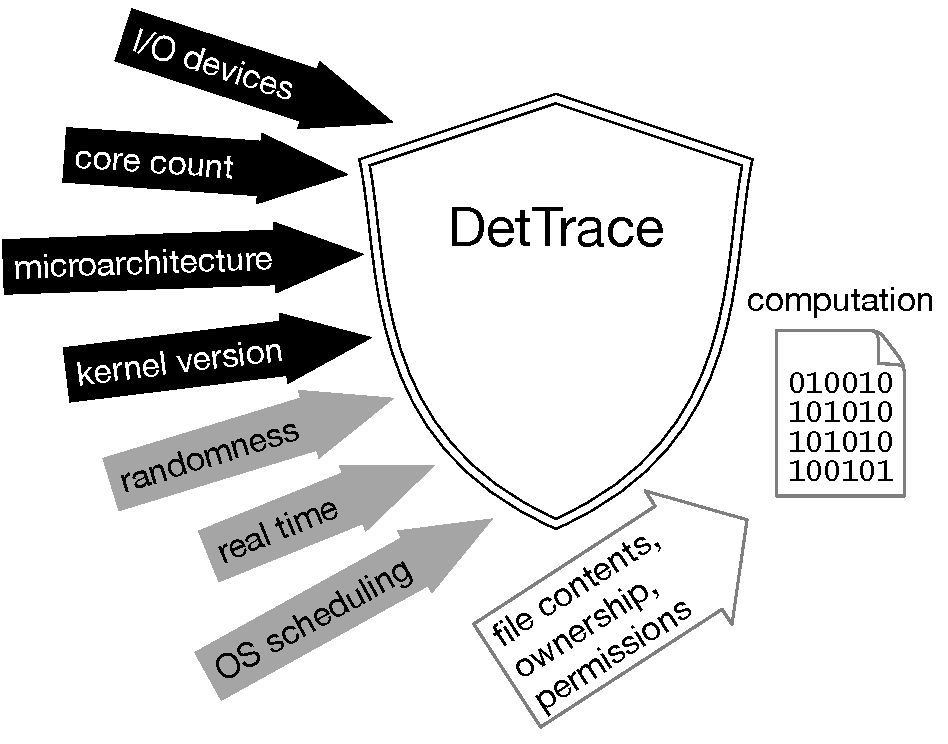
\includegraphics[width=0.95\columnwidth]{dettrace_figures/container-abstraction-shield.pdf}
  \caption{ \shrink{\vspace{-1mm}}
    \dettrace containers abstract away both sources of nondeterminism (gray arrows) and nonportability (black arrows), making a \dettrace computation a pure function of its initial file state.
  \shrink{\vspace{-2mm}}}
  \label{fig:abstraction}
\end{figure}


Ultimately, a \dettrace container runs as a pure function of the
container configuration and initial filesystem state.
%
File contents affect the computation, but file metadata is only
partially visible.
% Two runs where, say, the contents of a file on disk vary may produce different output.
%
% (which includes file contents, {some aspects of ownership and permissions},
%% \rn{These days I thought that external ownership was mapped
%%   onto a different ownership model? (root/nogroup)  Tweaked this slightly.}
% but excludes other metadata like timestamps and inodes)
%
Two runs where only the \code{mtime} of a file varies will produce the same output, but a permissions
change can affect output.
%% \new{because \dettrace presents identical, canonical modification
%% times at the beginning of container execution, and
%% deterministically computed ones thereafter.}
%
\autoref{fig:abstraction} illustrates what constitutes an \emph{input}, \ie{} what can induce output changes in a \dettrace computation.

Existing container technologies (like Docker) do not provide reproducibility: they are neither deterministic nor portable, as many details of the host OS and processor microarchitecture are directly visible inside the container. Virtual machines offer stronger hardware abstraction but lack determinism and are also quite heavyweight. We believe that the \dettrace reproducible container abstraction delivers significant advantages over existing approaches for domains like building and testing software where reproducibility is critical.


\section{Reproducibility Requirements for Linux and x86-64}
% \section{Linux-x86 Reproducible Requirements}
\label{sec:repro-reqs}
% ================================================================================

Code running inside our user-space reproducible container has access to two major interfaces: the x86-64 instruction set and the Linux system call API. Because we place no restrictions on code in the container, it can contain arbitrary instructions and attempt arbitrary system calls. Inspired by the Popek and Goldberg virtualization requirements \cite{Popek:1974:FRV:361011.361073} which define the requirements to provide a virtual machine abstraction, we define the set of requirements for reproducibility. We analyze each documented x86-64 ISA instruction\footnote{There are some undocumented x86-64 instructions \cite{breaking-x86}. Handling these would be an interesting avenue for future work.} and system call to see if it can be a source of irreproducibility, and under which conditions if so. Of particular importance is identifying \emph{critical} members of an interface---those which permit irreproducibility but which cannot be reliably detected during execution. Any \emph{critical} instruction or system call could silently introduce irreproducibility.

Our use of \code{ptrace} means that we see all system calls made from the
container, so there is no potential for a critical system call (we also handle
vDSO calls, see \autoref{sec:time}). If a given system call is a source of
irreproducibility, there are many potential mitigations: wrapping the syscall or
replacing it entirely with a deterministic counterpart
% behavior with a reproducible result
(like time calls), converting it into a nop (like sleep calls), or not supporting it and throwing a (reproducible) container-level error.

There are many sources of irreproducibility within the latest x86-64 instruction set \cite{intel-sdm}. Privileged instructions are often irreproducible but will raise an exception in our user-level container. Some irreproducible user-level x86-64 instructions are difficult, though possible, to trap. \code{rdrand} and \code{rdseed} return random bits from a hardware entropy source, and can be trapped at the hypervisor level via the VT-x extensions, but not from ring 0.  Instructions like \code{rdpmc} (read from performance counter) are sometimes accessible from user-space but can be configured to cause traps via appropriate kernel settings.

Some floating-point instructions like \code{cvtsd2si} (which converts a double
to an integer) are documented as having ``unpredictable behavior across
different processor generations'' with certain instruction encodings. We have
not investigated the extent of this behavior, but, by compromising portability,
it is a potentially critical source of irreproducibility.

%Load instructions can return different values on different runs of a parallel program, though \dettrace's sequential execution mitigates this issue. Other instructions like \code{cpuid} are deterministic on a given machine but vary across machines and are thus also a source of irreproducibility. Intel chips from Ivy Bridge onwards support trapping on \code{cpuid} instructions, making them non-critical.

\label{sec:tsx-intro}
\mypara{TSX Irreproducibility}
Ultimately, we found just one family of definitively critical instructions: the
TSX instructions used for transactional memory and lock elision (also noted by \cite{mozilla-rr-tr}). A transaction
can abort for a variety of reasons, some of which---like the arrival of a
timing interrupt---are highly irreproducible. A program can monitor its own
aborts via the abort handler registered with the \code{xbegin} instruction, and
perform irreproducible computation as a result. While the presence of TSX can be
hidden by crafting the return value of \code{cpuid}, an invalid or adversarial
program can ignore \code{cpuid} and run these instructions anyway. We are not
aware of any ability to trap on the execution of TSX instructions, though
Intel's microcode updates that disabled prior buggy versions of TSX \cite{tsx-disable} show
that software configurability does exist on some level. Hardware support for
trapping critical instructions is necessary for efficient and complete
detection, because the hardware knows definitively what instructions a program
is executing. Detecting the presence of \code{xbegin} in an adversarial program
is impractical: the program may jump into the middle of an
otherwise-valid instruction or employ self-modifying code to obfuscate its
behavior beyond the reach of static binary analysis. Dynamic analysis or
emulation can in principle catch such behavior, but only at a prohibitive
runtime cost.

Because current hardware does not allow our \dettrace prototype to trap \emph{all}
irreproducible instructions, we rely on programs being well-behaved enough not to
execute illegal or missing instructions (i.e., respecting the output of
\code{cpuid}).
%
%% While our current \dettrace prototype does not trap on all of the sources of
%% irreproducibility we are aware of (see \autoref{sec:insns}),
Nevertheless, our characterization of Linux system calls and x86-64 instructions
is a useful yardstick for work towards 100\% reproducible containers
that are robust against even adversarial programs.


\section{\dettrace Design}
% ================================================================================

\dettrace combines a lightweight sandboxing container with system call
interception to achieve reproducibility enforcement for arbitrary
Linux programs. \dettrace achieves this function while meeting our
design goals: a pure-software user-space solution, supporting
unmodified binaries, requiring no privileged (root) access, and
requiring no record and replay. \dettrace uses standard Linux container features: user, PID, and mount
namespaces, bind mounts and \code{chroot}. These mechanisms help to insulate programs in the container from programs and files outside it.

 \dettrace uses \code{ptrace} to intercept all system calls
made by code running in the container. The Linux ptrace mechanism allows one process (the {\it tracer}) to monitor the execution of another process (the {\it tracee}). The tracer can intercept the tracee's system calls (both before they reach the kernel and before they return to the tracee), signals, and more. The tracer can also read and write tracee memory and registers. Since the tracer is its own process, it is well-isolated from tracee faults (and vice-versa). However, extra context switches are required on intercepted events to jump to the tracer each time. In \dettrace, system calls with reproducible semantics are permitted through, while those with irreproducible
effects are either wrapped reproducibly or are identified as unsupported, triggering a runtime error.

\begin{figure}[t]
  \centering
  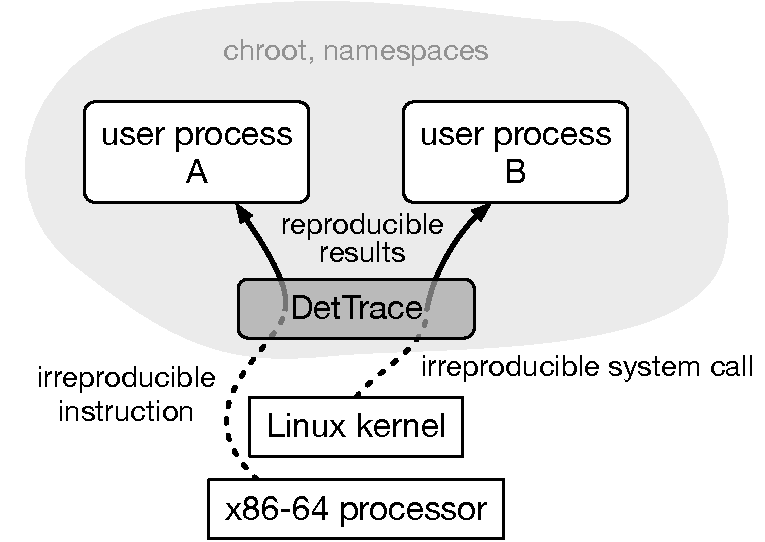
\includegraphics[width=0.95\columnwidth]{dettrace_figures/dettrace-architecture.pdf}
  \caption{High-level overview of \dettrace's organization. The unshaded blocks (processor, kernel and user programs) are completely unmodified.}
  \label{fig:arch}
\end{figure}


%\note{Trusted Code Base  \rn{I'd like to say something about this if there's room.}}


Next we detail sources of irreproducibility and describe how \dettrace renders each one reproducible. For simplicity, we use the term ``user process'' to refer to a process running inside a \dettrace container.

\subsection{Process, User and Group IDs}
\label{sec:ids}
% ~~~~~~~~~~~~~~~~~~~~~~~~~~~~~~~~~~~~~~~~
Thanks to our process namespace, processes inside our container receive unique PIDs that are independent of the world outside the container. A user process cannot name any process outside the container.  As user processes are created and terminated deterministically, and Linux allocates PIDs in each namespace sequentially, PIDs inside the container are naturally deterministic.
We similarly leverage uid and gid namespaces to similar ends. The first user process starts with root privileges, and can change identity via \code{setuid}.


\subsection{OS-Generated Randomness}
\label{sec:random}
% ~~~~~~~~~~~~~~~~~~~~~~~~~~~~~~~~~~~~~~~~

A Linux user process can request randomness from the OS via the \code{getrandom} system call, or by reading from the special \code{/dev/random} or \code{/dev/urandom} files. \dettrace intercepts \code{getrandom} system calls and fills the specified user buffer with values generated from a simple LFSR pseudorandom number generator. Similarly, \code{/dev/random} and \code{/dev/urandom} are named pipes to which \dettrace writes values from our PRNG. The PRNG seed can be specified when invoking \dettrace, to introduce randomness in a controlled way. User processes can also obtain randomness via the x86-64 instructions \code{rdrand} and \code{rdseed}, discussed later in \autoref{sec:insns}.

Some applications require true randomness for security reasons. \dettrace can provide such applications with direct access to, \eg, the real \code{/dev/urandom} and optionally log the values read to preserve reproducibility.


\subsection{Time and Clocks}
\label{sec:time}
% ~~~~~~~~~~~~~~~~~~~~~~~~~~~~~~~~~~~~~~~~
A variety of system calls return some form of timing information. For system calls that report wall clock time directly (like \code{gettimeofday}) \dettrace reports instead reproducible logical time values. For logical time, \dettrace uses {a count of the number of time calls performed by a user process}. This ensures that time monotonically advances between calls, which is important for some user programs which check timing behavior.
%Omar: I cannot find one of the top of my head, I know they exist though.

To enable high-resolution timing, Linux uses the virtual Dynamic Shared Object (vDSO) mechanism to implement timing system calls like \code{gettimeofday}. For performance reasons, these system calls are implemented as library calls and are thus not intercepted by \code{ptrace}. While Linux's \code{LD\_PRELOAD} mechanism is a natural choice for intercepting library calls, it is incomplete in small but important ways. First, it doesn't support statically-linked binaries. Second, a process can find the vDSO library within its address space (via \code{getauxval}) and directly call a vDSO function; indeed, \code{libc} does just this in its \code{mkstemp} function. To ensure airtight interception of vDSO calls, \dettrace instead, just after each \code{execve} system call, replaces the vDSO library code with our implementation where each vDSO function makes a direct system call---which is duly intercepted via \code{ptrace}. We furthermore make the \code{vvar} page unreadable to prohibit any access to the raw nondeterministic data that vDSO timing calls use. While replacing vDSO calls with normal system calls incurs a performance penalty, we plan to extend our vDSO library to handle the timing calls directly in a future version of \dettrace.

The x86 \code{rdtsc} instruction returns timing information in the form of
the current cycle count. Fortunately, \code{rdtsc} can be trapped and emulated
reproducibly, see \autoref{sec:insns}. Filesystem timestamps are a final source
of timing information which we discuss in \autoref{sec:timestamps}.
%
With nondeterministic parallelism, racing threads can recreate high-resolution clocks, but our deterministic scheduling renders this moot \cite{aviram_determinating_2010}.


\subsection{Signals and Timers}
\label{sec:sig}
% ~~~~~~~~~~~~~~~~~~~~~~~~~~~~~~~~~~~~~~~~

Signals are a prime source of irreproducibility as their arrival is typically asynchronous. In principle, signal generation and delivery can be made fully reproducible via a reproducible logical clock, as with deterministic shared memory synchronization \cite{kendo}. However, we have not found this necessary for our current workloads. Instead, \dettrace provides reproducibility for a subset of Linux signals. First, \dettrace does not support sending signals between user processes. It is important, however, that a user process can send itself signals. Some such signals are naturally reproducible: \code{SIGSEGV}, \code{SIGILL} and \code{SIGABRT} act like ``precise exceptions'' that halt program execution at a well-defined, reproducible state.

Timers, requested via system calls like \code{alarm}, are another common source of self-signals. To render timer expiration reproducible, timers in \dettrace expire ``instantaneously,'' invoking a signal handler if appropriate.
% include-if-space
We convert signal-generating timer calls (like \code{alarm}) into a \code{pause} system call that blocks the user process. Then, the tracer sends the necessary signal to the user process, invoking a registered signal handler if appropriate. This causes the \code{pause} call to return, and the user process resumes execution. The timer call never reaches the OS, but is instead emulated by the tracer.


\subsection{Files and Directories}
\label{sec:files}
% ~~~~~~~~~~~~~~~~~~~~~~~~~~~~~~~~~~~~~~~~
Files and directories are a rich source of irreproducibility, due to a complex API and extensive metadata. Our first step in providing a reproducible abstraction for files and directories is to isolate the view of the host filesystem that a user process has, accomplished via the \code{chroot} system call. \dettrace can also be nested inside standard containers like Docker to provide stronger filesystem isolation from the host.

File and directory \textbf{ownership and permissions} are inputs to a \dettrace computation (\autoref{fig:abstraction}). The Linux namespace controls the mapping from uid/gid inside the namespace to uid/gid on the host machine; this mapping is also part of the input to \dettrace.
By default, we map the current user account to \code{root} inside the container, and all others to \code{nobody}/\code{nogroup}.
%
%In contrast, Docker by default uses host ownership in volume mounts, making it easy to accidentally chown files to the host's root. % jld: while true, I think the comparison with Docker is distracting as this section is more about what DT does
% RN: Footnote version causes bad formatting:
% \footnote{\auditme{This differs from Docker's default approach, which does not reinterpret permissions in volume mounts (leading to files accidentally changed to root ownership on the host system).}}.

The order in which \textbf{directory entries} are returned is under the control of the filesystem implementation. To make the \code{getdents} system call reproducible, \dettrace sorts directory entries by name before returning them to the user process.

%\rn{For large directories, it would make sense to cache this information, but we do not currently do so.}

The \textbf{read} and \textbf{write} system calls have irreproducible semantics, as they may read/write arbitrarily fewer bytes than requested. While in practice we have never seen such ``partial'' operations on regular files, they do regularly arise when accessing pipes. To render these system calls reproducible in all cases, \dettrace automatically retries partial reads and writes until they process the requested number of bytes, or a read returns EOF. This is accomplished by decrementing the user process program counter to rerun the system call instruction, and adjusting the arguments to, \eg{}, tell the current \code{read} to continue where the previous \code{read} ended.

% \rn{I believe we need a large table somewhere for all this ``X maps to Y'' information....}

\textbf{Inodes} are unique identifiers for a file or directory within a filesystem mount. The \code{stat} family of system calls report inodes to a user process, and simply reporting a fixed value is insufficient as many user processes compare inode values to quickly identify identical files. Instead, \dettrace maintains a mapping from real (irreproducible) inodes to reproducible virtual inodes. Special care is needed to identify when a new file $f$ is created, as the OS may recycle a real inode for $f$ but \dettrace must allocate a new virtual inode to preserve reproducibility (see file timestamp discussion, next).


%% \jd{Scrapping this as it's too much detail. If it were to be in the paper, it should be in some kind of Grab Bag section}
%% \dettrace supports the \code{ioctl} system call, restricted to basic commands which are reproducible and are required for most programs to function, \eg{}, setting or querying terminal width.
%% \rn{What does ``restrict'' mean---errors or canonical values?  Seems we needa
%%     more discussion of our terminal policy here in general.}

\label{sec:timestamps}
\textbf{File timestamps} present a notion of time to user processes which, unfiltered, could be used to reconstruct an irreproducible clock. Thus, \dettrace virtualizes file timestamps. On Linux, each file or directory has three associated times: time of last content modification (mtime), time of last access (atime) and time of last content or metadata modification (ctime). In \dettrace, we always report atime and ctime as 0. However, we found that always returning a fixed value for mtime falls afoul of sanity checks in many programs. For example, \code{configure} from GNU Autotools checks for clock skew by creating a new file, then comparing its mtime to that of an existing file, raising an error if the mtimes don't make sense.

\dettrace implements a mapping between real inodes and virtual mtime, allowing for a reproducible, but sensible, response from system calls like \code{stat} that report mtime. Whenever a user process \code{open}s a file, before the \code{open} call reaches the kernel we check whether a file exists at the specified path. Before the \code{open} call returns to the process in the container, we identify the underlying real inode by examining the \code{/proc} filesystem to obtain the path and real inode of the newly-created file descriptor. By examining the path both before the \code{open} call reaches the OS and afterwards, we can reliably identify when new files are created. If the file was newly created, we assign its mtime as the current virtual mtime, and increment the current virtual mtime. Otherwise, the file existed in the initial container image and we assign it a virtual mtime of 0. Writes to a file do not currently update its virtual mtime because we have not found this necessary in our workloads, however this could easily be added to provide more realistic-looking virtual mtimes.

For \code{stat} calls, we consult our {\em real inode}$\rightarrow${\em virtual mtime} map to report mtime appropriately.
Any inode without an entry in the table gets a virtual mtime of 0, as it must have existed as part of the initial container image. Our lazy population of inode maps assigns reproducible virtual inodes and mtimes to every file in the container, while avoiding the need to index the entire container image at launch.


\subsection{Reproducible Scheduler}
\label{sec:multiproc}
% ~~~~~~~~~~~~~~~~~~~~~~~~~~~~~~~~~~~~~~~~
\dettrace supports multiple concurrent processes by sequentializing system call execution, and allowing processes to run in parallel for other operations. Our tracer makes scheduling decisions at system calls, process spawn, and process exit.
%These are all possible preemption points. Otherwise, the current process continues running.

\begin{figure}[t]
  \centering
  \shrink{\vspace{-2mm}}
  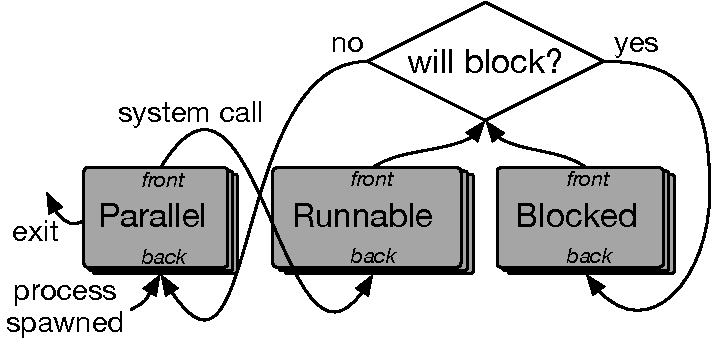
\includegraphics[width=0.95\columnwidth]{dettrace_figures/scheduler.pdf}
  \caption{State transitions for a user process in the \dettrace scheduler.
    \shrink{\vspace{-2mm}}}
  \label{fig:scheduler}
\end{figure}

\dettrace implements a reproducible scheduler, which consists of three queues. The \emph{Parallel} queue contains the processes currently running in parallel, and the other queues contain the processes that currently need to be scheduled for sequential system call execution. As \autoref{fig:scheduler} shows, processes begin their lives at the back of the \emph{Parallel} queue. The process at the front of the \emph{Parallel} queue moves to the back of the \emph{Runnable} queue when it needs to do a system call. The process at the head of the \emph{Runnable} queue is allowed to perform a system call next, if this system call will not block then the process returns to \emph{Parallel}, if it will block then the process moves to the end of \emph{Blocked} queue and will be revisited later. The process at the front of the \emph{Blocked} queue is then consulted to see if its system call will still block, and it moves to \emph{Parallel} or back to \emph{Blocked} accordingly.

%As \autoref{fig:scheduler} shows, a user process starts out in the \emph{Parallel} set and is allowed to run until it arrives at a system call or begins the exit sequence. The scheduler works by waiting on the parallel processes to see if any need to do a system call. Once the tracer is notified that a process needs to do a system call, the process is moved from the \emph{Parallel} set to the \emph{Runnable} deque. The tracer works by trying the system calls for all processes in the \emph{Runnable} deque, then the \emph{Blocked} deque,  and then waiting on the parallel processes for a finite amount of time to see if any parallel processes now need to do a system call.
%This is repeated until all processes have exited. When a process initiates exit under ptrace, it notifies the tracer. When the tracer receives this event, it detaches the process and removes the process from the \emph{Parallel} set so that the process can exit normally on its own.

% jld: too much detail here
%When a process $p$ attempts to exit (either cleanly or
%uncleanly), the tracer is notified. At this point, $p$ is stopped but still
%exists. Under ptrace, resuming $p$ at this point causes it to wait until all of
%its children have also exited, which can deadlock under \dettrace's sequential
%scheduling. Thus, we mark $p$ as \emph{Finished} and track the process
%tree so we can determine when all of $p$'s children have
%exited. Then it is safe to run $p$ so it transitions to the \emph{Exited} state
%and is removed from the \dettrace scheduler (and the underlying OS).

\subsubsection{Blocking System Calls}
\label{sec:blocking}
System calls that may block exhibit a potential for deadlock with \dettrace's sequential system call execution. \dettrace avoids deadlock by identifying in advance (and, of course, reproducibly) whether a system call may block. On any given potentially-blocking system call $s$ from a process $p$, $s$ can either succeed immediately, or $p$ must wait until some event in another process enables $s$ to complete. If the former, we execute $s$, move $p$ to the \emph{Parallel} set, remove it from the queue it was on, and resume $p$ in parallel. If the latter, we preempt $p$ by moving it to the \emph{Blocked} queue.

To detect whether a system call will block or not, we transform blocking calls into non-blocking ones, \eg{} a \code{wait4} call is modified to use the \code{WNOHANG} flag.
%All system calls that may block encountered so far have a mechanism to convert into non-blocking.
When the non-blocking system call returns and indicates the resource is not available, we preempt the process and move it to the end of the  \emph{Blocked} queue. We reset the process state to retry the system call in the future.

%Because blocking queries resolve reproducibly, \dettrace can support ostensibly-nondeterministic system calls like \code{poll} and \code{select} operating on pipes and regular files

Some system calls, like a \code{write} to a pipe, may unblock one or more other processes. We do not track such dependencies between processes; when process $p$ writes to a pipe we do not know precisely which \emph{Blocked} processes (if any) this will unblock.  But, because the scheduler iterates fairly over \emph{Runnable}, \emph{Blocked} and \emph{Parallel} processes, any unblocked process will eventually run.

%\fixme{A more sophisticated dependency tracking technique could track fine-grained resource dependency between processes, but we found our current implementation to be sufficient.}

\subsection{Threads}
\label{sec:thread}
The \code{ptrace} API for threads and processes are identical, allowing \dettrace to support threads with few extensions to the scheduler. Threads within a process are sequentialized to render shared memory interactions reproducible.

% include-if-space
%The biggest challenge for thread support is supporting the \code{exit\_group} system call. When an \code{exit\_group} is triggered, all threads in the current \emph{thread group} will exit. A thread group $TG_{p}$ is a set containing the parent thread (a process with PID $p$) and all its child threads. Just like the process exit procedure described previously, $p$ cannot exit until all its child threads have exited. Therefore, we track thread group members. When \code{exit\_group} is invoked, we schedule all child threads in $TG_p$ for exit. When all child threads have exited, $p$ is marked as \emph{Finished}. When $p$'s child processes have \emph{Exited}, then $p$, too, can transition to the \emph{Exited} state.

The \code{futex} system call is Linux's implementation of fast, userspace locks.  We treat \code{futex} wait calls like any other blocking system call (\autoref{sec:blocking}). If threads busy-wait instead of blocking, our sequential scheduler fails to make progress, which is one reason a program may be incompatible with \dettrace (\autoref{sec:unsupported}).

\subsection{CPU Instructions}
\label{sec:insns}
% ~~~~~~~~~~~~~~~~~~~~~~~~~~~~~~~~~~~~~~~~

% \jd{would be good to document when various hardware features were introduced. General rdtsc interception via prctl landed in Linux 2.6.26 in July 2008. Not sure when the x86 feature was first introduced, but it seems to predate 2.6.26 significantly as seccomp was already disabling rdtsc in previous versions of Linux.}

While irreproducible CPU instructions cannot be
intercepted through ptrace, recent x86 hardware provides
mechanisms for intercepting many irreproducible instructions
(\autoref{sec:repro-reqs}). Our current \dettrace implementation
intercepts the \code{rdtsc} and \code{rdtscp} instructions, which
return a count of current cycles, via the \code{prctl} system call.
%Using the \code{prctl} system call,
%we ask the kernel to raise a segmentation fault whenever
%\code{rdtsc[p]} execute. To differentiate between a segmentation fault
%caused by a program memory error versus a faulting \code{rdtsc[p]}, we
%use ptrace to check the instruction that triggered the fault.
For \code{rdtsc[p]}, we overwrite their nondeterministic result with
a linear function of \code{rdtsc[p]} instructions executed so far.

Additional irreproducible instructions include TSX instructions,
\code{rdrand}, \code{rdseed}, and \code{cpuid}.  Serendipitously, the
latter provides a solution to the former: we use \code{cpuid} interception to
report the absence of TSX and hardware randomness support, as
described in \autoref{sec:tsx-intro} (while adversarial programs can try
running them anyway, supporting such programs is not our target).
%
While hypervisors have long been able to intercept \code{cpuid},
Intel's Ivy Bridge
microarchitecture introduces a ring 0 mechanism that the Linux kernel
(starting with 4.12) exports to user-space.
%

With an Ivy Bridge or newer machine, we can achieve forward-portability when
rerunning a job: pinning the reported system information, while
supporting subsequent processors.
%
We also simplify the hardware details presented to the user process, for example
listing a single core and canonical cache size.  This further increases the
equivalence class of machines which {\em must} observe the same answer for a job.

Older Intel architectures, such as Sandy Bridge, lack user-space \code{cpuid}
interception, but they {\em also lack} \code{rdrand} and TSX.  Therefore \dettrace can still run reproducibly on
these older machines, but the portability guarantee ranges over a much smaller
class of machines because we cannot hide \code{cpuid} information.

\subsection{Unsupported Operations}
\label{sec:unsupported}
% ~~~~~~~~~~~~~~~~~~~~~~~~~~~~~~~~~~~~~~~~
Here we describe some limitations of our current \dettrace prototype. If a user process attempts to use one of these features, \dettrace raises an error. \autoref{sec:unsupportedPkgs} evaluates in more detail the number of Debian packages that fail to build due to these reasons.

\dettrace does not support \textbf{busy-waiting} threads because our scheduler performs context switches for threads only at thread creation/exit and system calls. \textbf{Sockets} are also not supported, as arbitrary socket use for network communication is a significant reproducibility challenge. We plan to investigate limited forms of socket communication, \eg{} as interprocess communication within our container, that can be rendered reproducible.

%% \jd{keeping this in a comment as it's good documentation}
%% The Linux kernel treats threads and processes quite similarly with some subtle but
%% important differences. One disadvantage of ptrace is it's poor support for threads,
%% with a difficult to use API and little documentation. However, the scheduler outlined
%% for processes can be extended to work with threads. With the following additions:
%% \begin{itemize}
%% \item Thread Id: The thread ID should be used instead of the process id, this information
%%   is readily available from the return value of ptrace.
%% \item Thread Group Id (TGI): Threads in the same process share the same TGI. In
%%   a scheduler which may have threads from multiple different processes, the TGI is
%%   needed properly exit all threads due to certain events (see next bullet point).
%% \item Tearing down threads: If any thread in a thread group calls either exit group or
%%   execve, all threads within that TGI will exit immediately. Thus the scheduler must
%%   know to mark all these threads as ready for exiting and schedule them all to to have
%%   the kernel clean up their state.
%% \end{itemize}

%% Our prototype has minimal support for threads due to missing implementation for TGI and
%% tearing down threads semantics. Thus we cannot run Java programs, which run to
%% completion but appear to dead lock on a call to exit group(2) since the scheduler does
%% not attempt to exit threads in the same TGI. Programs which do not tear down threads
%% through exit group or execve run deterministically as expected.




%% \rn{Ryan Newton's notes:}
%% \note{Blocking sequential semantics---what's our name/slogan for this?}

%% \note{Defining a determinism delta---a modification to the Linux syscall and
%%   file system semantics.  But different that dOS and user-space.}

%% \note{No synthetic schedule...  merely a sequential schedule}



\subsection{System Call Modification}
%================================================================================
\label{sec:impl}

%In the prior section, we described our algorithmic solutions for how to
%transform Linux x86-64 into a deterministic platform.
%
%In this section, we turn to the implementation details of our ptrace system call interception.
%optimizing interception, \rn{and limitations of the current prototype}.


% \label{sec:ytrace}
% ~~~~~~~~~~~~~~~~~~~~~~~~~~~~~~~~~~~~~~~~
%% \rn{I think we can have a section that explains what we ideally want to do, how
%%   systems like Windows picoprocesses accomplish it, and how ptrace enables it
%%   portably but somewhat awkwardly and idiosyncratically.}

\begin{figure}[t]
  \centering
  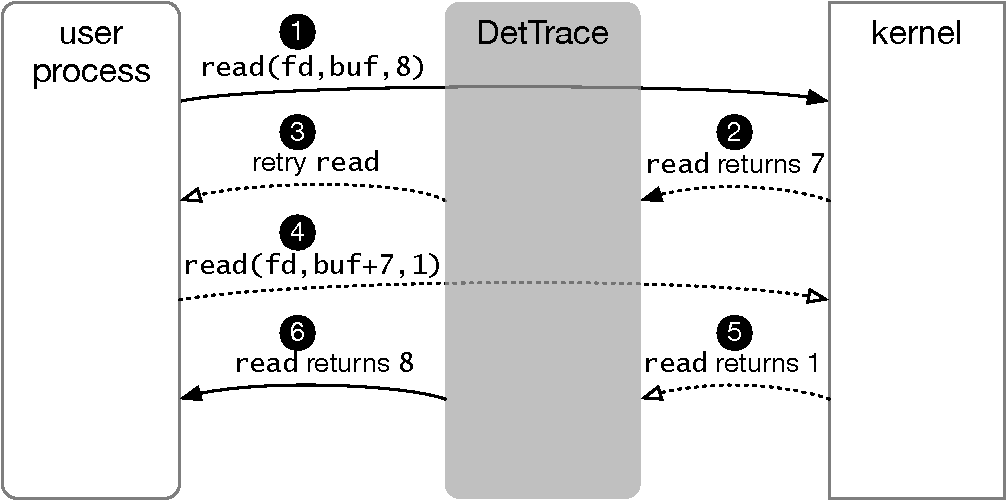
\includegraphics[width=0.95\columnwidth]{dettrace_figures/read-retry-dance.pdf}
  \caption{To render the \code{read} system call reproducible, \dettrace retries \code{read} operations that do not return the requested number of bytes. The solid arrows indicate what the user process perceives to have occurred. The dashed arrows indicate extra operations \dettrace undertakes to provide the illusion of reproducibility.}
  \label{fig:read-retry-dance}
\end{figure}

% include-if-space
\dettrace uses ptrace to intercept but then skip certain system calls, \eg{} timer calls that \dettrace emulates internally (\autoref{sec:sig}). While one cannot directly skip a system call with ptrace, one can indirectly skip it by replacing the system call number before it is examined by the kernel. We use \code{time} as a convenient ``NOP'' system call that takes no arguments and always succeeds.

We can leverage system call interception to arbitrarily modify, replay or inject new system calls. As a more involved example, \autoref{fig:read-retry-dance} illustrates the system call injection we perform when a user process performs a \code{read} system call that requests 8 bytes though the kernel initially returns only 7. \dettrace adjusts the \code{read} arguments to fill in the user buffer with the remaining bytes and resets the PC to perform another \code{read}. Once the user buffer is full (or we reach EOF), the user process is allowed to continue past the \code{read} call, with the buffer seemingly filled on the first try.

% include-if-space
Sometimes a system call requires that we allocate memory in the tracee address space. For example, the \code{utime} system call sets the atime and mtime for a file at a given path. If the times are specified as \code{null}, then the kernel sets the atime/mtime to the current time. To avoid the kernel setting irreproducible timestamps, \dettrace needs to allocate a timestamp struct in the tracee address space, initialized with reproducible timestamps, and call \code{utime} with this struct as an argument. To this end, \dettrace allocates a page of memory in each tracee's address space after each \code{execve} system call. Our custom timestamp struct is allocated from this page, to avoid perturbing the tracee's heap or stack.


%% System call modification:
%%   Ptrace allows us to change the arguments of system calls before the system call is
%%   executed. Consider the utimensat system call. Which sets the timestamp for a file,
%%   if NULL is passed as the time, the file's timestamp is set to the current time. To
%%   stop this nondeterministic behavior we change this argument to point to a
%%   deterministic time instead.

%% System call replaying:
%%   Having access to a process’ instruction pointer register, allows to rewind execution of a
%%   process.
%%   All instructions on x86-64 (list them here) capable of calling a system call are
%%   two bytes long. So setting the RIP register to $RIP - 2$ allows us replay the
%%   a system call. Arbitrary arguments and memory may be modified between calls for a
%%   flexible and powerful mechanism.

%% System call injection:
%%   system call replaying is a special case of this. We may inject arbitrary system calls
%%   during any system call interception event. By merely changing the registers we can call
%%   arbitrary system calls on the tracee. Technically a system can be injected at any ptrace
%%   even where the tracee is stopped. This more complicated as it requires rewriting
%%   memory with a system call instruction.


%\subsection{Optimizations}
%~~~~~~~~~~~~~~~~~~~~~~~~~~~~~~~~~~~~~~~~
%\label{sec:opt}

% ~~~~~~~~~~~~~~~~~~~~~~~~~~~~~~~~~~~~~~~~
\subsection{Improving performance with seccomp-bpf} \label{sec:seccomp}
By default ptrace stops the tracee for every system call twice, but Linux's \code{seccomp-bpf} mechanism allows for selective system call interception, avoiding overhead on system calls that are naturally reproducible in our environment (like \code{getcwd}). seccomp also allows the interception code, which runs before a system call reaches the kernel, to dynamically decide whether or not to intercept after the system call completes, further reducing overhead. Linux kernel versions $>= 4.8$ additionally optimize context switches by delivering a single event instead of separate pre-system-call and seccomp events. We support kernel versions $< 4.8$ by falling back to the slower implementation.


\section{Experimental Methodology}
\label{sec:methodology}
%================================================================================

We ran our package build evaluation using Debian 7
(Wheezy) packages, a stable version first released in May 2013 which contains
\BaselineTotalPkgCount packages total. We chose this version of Debian to avoid
confounding effects from the efforts of the Debian Reproducible Builds
project, which began in late 2013. We wanted to capture an accurate
pre-DRB picture of the Debian package ecosystem.


We build our packages on CloudLab \code{c220g5} nodes, where each node has
two Intel Xeon Silver 4114 Skylake processors, each with 10 cores (20 threads) running at
2.2GHz, and 192GB of RAM. These processors support
interception of the \code{cpuid} instruction (\autoref{sec:insns}). We use the full
seccomp-bpf optimizations. Each node runs Ubuntu 18.04 LTS with the Linux 4.15 kernel.

For our bioinformatics workflows, we used \code{RAxML} 8.2.10 with AVX support~\cite{raxml}, \code{Clustal} 2.1 in \code{-ALIGN} mode~\cite{clustal} and \code{HMMER} 3.1b2~\cite{hmmer}.
%, \code{mothur} 1.39.5 in \code{make.contigs} mode~\cite{mothur}, \code{BWA} 0.7.10~\cite{bwa}.
We used TensorFlow v1.14 in our ML experiments, using the \code{alexnet} and \code{cifar10} tutorials \cite{tf-models-tutorials} to perform model creation, training and inference. Bioinformatics and ML workloads run on a machine with two Intel Xeon E5-2618Lv3 (Haswell) processors each with 8 cores (16 threads) running at 2.3GHz, and 128GB of RAM. The machine runs Ubuntu 18.10 with Linux 4.18.

\subsection{Verifying Reproducibility}
\label{sec:verifyRepro}

%\jd{figure here of Docker, reprotest chroot(s), apt-get build-dep, dettrace dpkg-buildpackage}
%
\mypara{Package builds} We build packages, both with and without \dettrace, inside a fresh Docker instance to easily control filesystem state.\footnote{\dettrace can also provide an
  isolated filesystem environment, but Docker provides easy
  image distribution across our cluster. \dettrace
  nests within Docker without issue.} Inside the container, we use a
slightly modified version of the
\code{reprotest} utility version 0.7.8 \cite{reprotest} from the DRB
project. \code{reprotest} builds each package twice, varying the
conditions for each build to exacerbate irreproducibility. We
configure \code{reprotest} to vary environment variables, build path,
ASLR, number of CPUs, time, user groups, home directory, locales, exec path, and
timezone. We turn off domain host, kernel, and file ordering as they are
not supported by the older version of Debian we're running our builds in.
Similarly, the umask variation would randomize file permissions which \dettrace does
not hide from user processes.

% include-if-space
By default \code{reprotest} chooses variations randomly; we modified it to use a consistent configuration for the first build of all packages, and a different consistent configuration for all second builds, so that
exactly the same environment is presented to \dettrace as in the baseline.
%
%For each package build, we first download the source package and install dependencies, and then run the build via \code{dpkg-buildpackage} either with \dettrace or without it (the \emph{baseline}).
% include-if-space
We create a \code{control-chroot} of a minimal Wheezy installation, downloading the source via \code{apt-get source}, then installing a package's dependencies via \code{apt-get build-dep} (referencing an on-disk mirror to avoid network requests and ensure consistency across builds). Finally we copy the \code{control-chroot} to create an \code{experiment-chroot}, thus guaranteeing the same starting image for both builds. \code{reprotest} takes these starting chroots for running \code{dpkg-buildpackage} with or without \dettrace. When using \dettrace, everything \code{dpkg-buildpackage} does runs under \dettrace, which includes compilation, running tests (if the package is configured to do so), and creating the final \code{.deb} package.
After both builds are complete, \code{reprotest} validates
reproducibility with bitwise comparison of the two \code{.deb} packages.
% include-if-space
\code{reprotest} calls another DRB tool \code{diffoscope} which compares two directories, checking for bitwise identical contents. If \code{diffoscope} reports no differences the package is deemed \emph{reproducible}, otherwise the package is deemed \emph{irreproducible}.

Under this Debian/\code{reprotest} configuration \BaselineStandardPkgCount,
 or \BaselineStandardPkgPct, of the total available packages build completely,
whereas \BaselineTimeoutPkgCount time-out after 30 minutes and \BaselineFailedPkgCount fail to build.  For the
evaluation in the next section, we focus on the set of \BaselineStandardPkgCount
packages that build in the baseline, whether reproducibly or
irreproducibly.
%
% Debian Wheezy packages represent an ideal opportunity for deploying \dettrace.
In fact, in a {stock} Wheezy system, \emph{zero} packages build
reproducibly because of timestamps embedded by \code{tar}. So we adjust our
driver script to unpack the deb packages using \code{dpkg-deb}, then run
\code{strip-nondeterminism} \cite{strip-nondeterminism} on the individual files, stripping
timestamps.
Finally, \code{diffoscope} can do a meaningful bitwise comparison. % include-if-space
The \dettrace builds do not require this workaround, as they are
naturally robust to timestamps.
%
With the tar-timestamp workaround, \BaselineStandardReproCount
(\BaselineStandardReproPct) packages are reproducible in a stock Wheezy
system.
%
The other \BaselineStandardIrreproCount packages require additional manual
intervention to achieve reproducibility. %Alternatively, \dettrace can provide reproducibility \emph{automatically} for the vast majority of packages supported by the prototype, as we demonstrate next.

\mypara{Bioinformatics} While we did not leverage an ad\-ver\-sar\-ially-irreproducible environment like \code{reprotest} for the bioinformatics tools, using \code{hashdeep} on the outputs from \code{HMMER} and \code{RAxML} revealed irreproducibility across consecutive runs on a single machine. We confirmed (using \code{hashdeep}) that the irreproducibility is removed when running under \dettrace. The \code{clustal} workflow appeared reproducible, both natively and with \dettrace.

\mypara{Machine Learning} To check the reproducibility of our TensorFlow workloads, we recorded the value of the loss function at each step during training. Unsurprisingly, these values are irreproducible when running natively, even with serialized TensorFlow (see \autoref{sec:eval-tf}), due to, e.g., randomization of the training set. \dettrace renders these workloads reproducible without any code changes.

\begin{table*}[t]
	\small
  \begin{center}
  \begin{tabular}{|c|c|c|c|c|c|}
  \hline
  % Nota bene: the "DT Unsupported" category is the combination of BuildFailed and DettraceFailed
  Given & DT Reproducible & DT Irreproducible & DT Unsupported & DT Timeout \\
  \hline
  % BEGIN AUTOGENERATED CONTENT
  % Run `./data/scripts/Bayes.hs --baselineCSV data/sosp2019/summary_baseline_standard.csv --dettraceCSV data/sosp2019/summary_dettrace_concurrent_standard.csv --narrowed`
  % in dettrace-experiments to generate this.
  BL Irreproducible (11,958) & 72.65\% (\BaselineIrreproDTReproCount) & 0\% (0)
                                   & 15.99\% (1,912)           & 11.36\% (1,358) \\
  BL Reproducible (3,803)    & 90.51\% (3,442)                        & 0\% (0)
                                   & 3.60\% (137)              & 5.89\% (224) \\
  \hline
  \end{tabular}

  \vspace{2mm}

  \begin{tabular}{|c|c|c|}
  \hline
  Given & BL Reproducible & BL Irreproducible \\
  \hline
  \dettrace Reproducible (12,130) & 28.38\% (3,442) & 71.62\% (\BaselineIrreproDTReproCount) \\
  \dettrace Timeout (1,582) & 14.16\% (224) & 85.84\% (1,358) \\
  \dettrace Unsupported (708) & 7.91\% (56) & 92.09\% (652) \\
  % END AUTOGENERATED CONTENT

  \hline
\end{tabular}
  \end{center}
  \caption{(Top) How build status changes moving from the baseline (BL) to \dettrace (DT), and from DT to BL (bottom). \dettrace automatically renders reproducible \BaselineIrreproDTReproPct of packages that are irreproducible in the baseline.}
  \label{tab:bayesian}
\end{table*}

\section{Evaluation}\label{sec:eval}
% ================================================================================
In this section, we describe our results using the \dettrace system with software builds, and bioinformatics and machine learning applications.


\subsection{Package Build Reproducibility}

Package builds can fall into one of four categories when building under \dettrace. Some package builds are \emph{reproducible} or \emph{irreproducible} as described in \autoref{sec:verifyRepro}. \emph{Timeout} packages do not finish building within 2 hours. We allot a high timeout for \dettrace to account for its performance overheads and to avoid eliding high slowdowns from our performance evaluation. Lastly, a package may be \emph{unsupported} for a variety of reasons we discuss in \autoref{sec:unsupportedPkgs}.


Of the \OurNarrowCount packages that \dettrace supports (\ie{} the build with \dettrace is neither \emph{unsupported} nor does it timeout), \dettrace is able to render every single package reproducible. This represents \OurReproLOC
(non-comment/non-blank) lines of code from over 3.3 million source files building under \dettrace.

\autoref{tab:bayesian} shows how package status changes when moving from the baseline to \dettrace and vice-versa, focusing just on those packages that build (reproducibly or irreproducibly) in the baseline. The top table shows what happens to baseline packages when run with \dettrace. For example, the first row shows that of the \BaselineStandardIrreproCount packages that are irreproducible in the baseline, \BaselineIrreproDTReproCount of them are automatically rendered reproducible by \dettrace.
% , and just \OurNarrowIrreproCount remain irreproducible.
Reassuringly, packages that are reproducible in the baseline never become irreproducible under \dettrace.

The bottom table in \autoref{tab:bayesian} shows, for a package with a given \dettrace status, what happens in the baseline. Packages that timeout or are unsupported by \dettrace are very commonly irreproducible in the baseline, suggesting these are more complicated builds.

% NB: The figures in the paragraph below are taken directly from the
% conditioned probability table (percentages reduced to one sig fig):
%
% (1)(a) 71.72%        (Given baseline Irreproducible -> DetTrace Reproducible)
% (1)(b) 7942 packages (Same as above)
% (2)    27.27% (Given baseline Irreproducible -> DetTrace DetTrace Unsupported)
%% If we consider an arbitrary package chosen that builds in the baseline, then the
%% odds of becoming reproducible are reduced by fraction of packages that hit
%% features not yet supported by the prototype: still, adding \dettrace is
%% 71.7\% % (1)(a)
%% likely to fix the problem (with
%% 7942 % (1)(b)
%% packages automatically going from irreproducible to reproducible) but
%% 27.3\% % (2)
%% likely to hit an unsupported feature.

%% \begin{figure*}[ht]
%%   \centering
%%   
\includegraphics[height=4cm]{dettrace_figures/placeholder.pdf}
%%   \caption{DRB packages. The \Red{WHICH} line indicates the baseline packages,
%%            while the \Red{WHICH} line indicates packages built with
%%            \dettrace{}.}
%% \end{figure*}

\subsubsection{Unsupported Packages}
\label{sec:unsupportedPkgs}
A total of \OurNarrowDettraceFailCount packages failed to build due to known \dettrace limitations. The  most frequently encountered issue was busy waiting, which arose for 876 Java packages (45.8\% of failures) that fail to build. The next most common reasons are socket operations (302 packages, 15.8\%), and sending intra-process signals (79 packages, 4\%). The rest form a long tail of miscellaneous system calls \dettrace does not yet support. Note our Java detection heuristic does not apply to other cases of busy waiting, which result in a \emph{timeout} instead.

%% OLD / ASPLOS submission 8/2018:
%% \fixme{Lack of thread support was by far the most common reason}, accounting for
%% \fixme{80\% of failures (2,441 packages)}. Other reasons are far rarer,
%% including support for sockets
%% \fixme{(257 packages)} and inter-process signals
%% \fixme{(92 packages)}. The rest form a long tail of
%% miscellaneous system calls and other implementation limits.

\subsubsection{Comparison with DRB}
\OurReproDRBIrreproCount of the packages that are reproducible under \dettrace are identified as \emph{irreproducible} in the current stretch release by DRB~\cite{drb-unrepro}. While those packages are newer than the Wheezy versions we use, the DRB effort has also categorized why these packages are irreproducible. Common reasons include build paths being captured in a build artifact, timestamps embedded in files and randomness affecting build artifacts. Though these issues have been resolved in hundreds of other packages, each package requires analyzing the cause of irreproducibility and getting patches accepted by maintainers. In contrast, \dettrace automatically makes a build immune to such variations.

\subsubsection{Comparison with Mozilla \code{rr}}
\label{sec:eval-rr}

Record-and-replay (RnR) systems are similar to \dettrace in needing to intercept sources of nondeterminism. However, record-and-replay systems do not directly facilitate reproducible builds, as opaque recording files do not enable one to inspect the source code of a package. Recordings also require storage, typically much more than pure source code. We undertook a small experiment with the latest version (5.2.0) of the \code{rr} tool, as it is the most robust RnR system we are aware of.  We selected 81 packages that build from source natively in Ubuntu 18.04 (to provide a more modern build environment for \code{rr} than Debian Wheezy), and tried building them with \code{rr}. Unfortunately, \code{rr} crashed on 46 of them due to a known bug with unsupported \code{ioctl} calls. Of the 35 packages that build with \code{rr}, the average runtime overhead was 5.8$\times$ (ranging from 3.3-22.7$\times$), comparable to \dettrace. Unlike RnR, \dettrace avoids opaque recordings and provides a human-readable audit trail from inputs to outputs.

\subsection{Package Build Correctness}\label{sec:correctness}

To validate the functional correctness of \dettrace, we used several of the packages built using our system to ensure they work correctly. For example, we built the popular 3D graphics package \code{blender} with \dettrace, installed the resulting \code{.deb} on a Debian wheezy virtual machine, and used the UI to render a sample project. We built the
core TeX/LaTeX packages using \dettrace and used them to build the paper you're reading.

To validate \dettrace's correctness on a complex software system, we first built the LLVM 3.0 compiler from source without using \dettrace. %using the version of \code{clang} (which we term \code{apt-clang}) installed from the standard \code{apt} package manager.
We ran LLVM's test suite via the \code{make check} finding that 5,594 tests pass, 48 expectedly fail and 15 are unsupported in this baseline configuration.
%We then repeated this experiment using \code{det-clang}, the \code{clang} package built using \dettrace instead, and received the same results from the LLVM test suite. As a third experiment,
We then ran the LLVM build under \dettrace (using a version of \code{clang} built with \dettrace as well) and received the same test outcomes. Given the complexity of the LLVM source code, we find these results with ``self-hosting'' LLVM encouraging evidence that software built using \dettrace functions correctly.

%Unfortunately, a thorough examination of correctness across all packages is not straightforward. Debian packages provide no standard way of seeing whether tests are run as part of the package build, let alone identifying the number of tests or their success rate. Extracting this information would require manually investigating the stdout/stderr output of each build.

\subsection{Package Build Portability}\label{sec:portability}
To evaluate \dettrace's portability, we perform package builds on two different machines with different microarchitectures and OS versions. One machine is our standard CloudLab node (described in \autoref{sec:methodology}) and the other has Intel Xeon E5-2620 v4 processors (Broadwell instead of Skylake) running Ubuntu 18.10 (instead of 18.04, Linux versions 4.18 and 4.15, respectively). We use the same \code{reprotest}-based build methodology to perturb the environment, and ensure that each build on each machine produces a bitwise-identical package. Due to time constraints, we randomly selected 1,000 packages reproducible with \dettrace. Every one built identically across the two systems.

% include-if-space
Achieving portability for these packages required one extension to \dettrace. We found that the size of a directory (returned by \code{stat}) varied across machines, though the directory contents were identical, were created via extraction from the same tarball, and the filesystem type and block size were the same. This behavior had not arisen across any of our previous experiments which used a single machine type, empirically illustrating the distinction between portability and determinism. \dettrace implements reproducible directory sizes by reporting sizes as a deterministic function of the number of directory entries.

\subsection{Package Build Performance}\label{sec:perf}
% ~~~~~~~~~~~~~~~~~~~~~~~~~~~~~~~~~~~~~~~~

%% \rgs{From Omar: I actually think you're better equipped to handle this section?}

%% \onl{package build performance:
%%   aggregate time to build all packages
%%   maybe aggregate user/system time as well
%%   CDFs of per-package real/user/system times}

\dettrace is designed for reproducibility, but is only moderately optimized for
performance overheads.
Considering builds in aggregate, \dettrace incurs an total \SlowdownRealMean slowdown in wall
clock time. \autoref{fig:slowdowns} shows a scatter plot for 860 randomly-selected \dettrace-supported packages, showing \dettrace's slowdown over the baseline (log scale) against the build's rate of system calls per second (as measured by \dettrace). We exclude builds that run for less than 5 seconds in the baseline, and we run just one package build per machine to avoid performance interference.
%Each baseline build runs pinned to a single core to allow us to measure \dettrace's overheads beyond that of process serialization.\footnote{In other experiments where the baseline is not pinned, it achieves only modest speedups because most builds do not use parallelism.}
We crop a few outliers from the plot to make it easier to read: 4 packages that perform more than 25,000 syscalls/second (the max is 82,533 for \code{the}) and exhibit slowdowns from 3.97-30.11$\times$, and 3 packages that run about twice as fast with \dettrace than in the baseline---though they appear to build correctly, \eg their internal tests all pass at the end of the build.

The light orange dots in \autoref{fig:slowdowns} show packages that do not use threads, while the dark blue dots show threaded packages. Overall, there is a positive correlation between \dettrace overhead and system call rate. Though there are just 76 threaded packages in this sample, they exhibit some of the highest slowdowns due to common futex operations being converted from blocking to non-blocking.

% the outlier with 63.7x slowdown is arpack++.

% how to compute this ``end-to-end'' wall clock time:

%% $ csvsql --query "select PACKAGE,BUILDSTATUS from '48,50,51,52_dettrace_standard' group by PACKAGE" data/big-runs/48,50,51,52_dettrace_standard.csv | csvgrep -c BUILDSTATUS -r "^reproducible|^unreproducible" > temp.csv
%% $ csvjoin -c PACKAGE data/big-runs/68-baseline.csv temp.csv > temp2.csv
%% $ csvsql --query "select PACKAGE,AVG(BUILDTIME_REAL) from 'temp2' group by PACKAGE" temp2.csv | csvstat -c "AVG(BUILDTIME_REAL)" --sum
%% 246,270.15

%% $ csvsql --query "select PACKAGE,BUILDSTATUS,AVG(BUILDTIME_REAL) from '48,50,51,52_dettrace_standard' group by PACKAGE" data/big-runs/48,50,51,52_dettrace_standard.csv | csvgrep -c BUILDSTATUS -r "^reproducible|^unreproducible" | csvstat -c "AVG(BUILDTIME_REAL)" --sum
%% 404,081

% >>> 404081 / 246270.15
% 1.6408038083381198


% ^ That 16 packages number can be verified like so:
%   csvsql --query "select COUNT(*) from 'all_slowdowns_48,50,51,52' WHERE SLOWDOWN_REAL > 12" data/slowdowns/all_slowdowns_48,50,51,52.csv

% (arithmetic)

\begin{figure}[t]
  \centering
  \shrink{\vspace{-3mm}}
  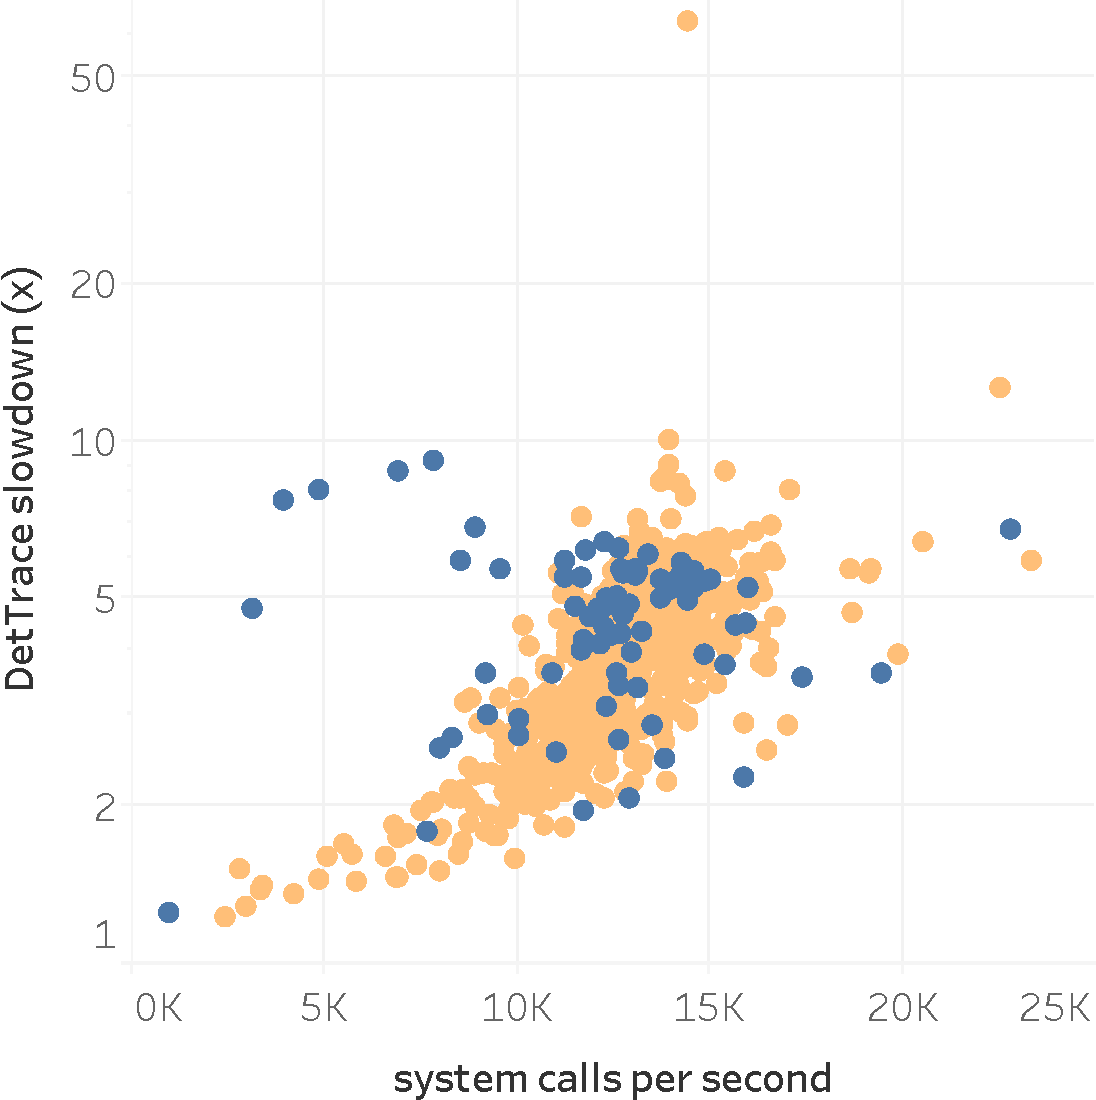
\includegraphics[width=0.8\columnwidth]{dettrace_figures/dt-overhead-syscalls-per-second.pdf}
  \caption{\dettrace overhead (y-axis, log scale) is largely driven by the rate at which system calls are performed (x-axis). Packages that use threads (dark blue dots) are typically slower than those that do not (light orange dots).}
  \label{fig:slowdowns}
\end{figure}


% include-if-space
%\mypara{Runtime events}
% ~~~~~~~~~~~~~~~~~~~~~~~~~~~~~~~~~~~~~~~~
%\dettrace counts a variety of relevant events on each run; the results are summarized in \autoref{tab:dettraceStats}. Data is drawn from all \OurNarrowDettraceReproPlusIrrepro packages that build with \dettrace.

We find that system calls are frequent in package builds, with over 800,000 in an average build (\autoref{tab:dettraceStats}).
%\dettrace also performs nearly 400,000 reads of user process memory on average, to extract pointer-based system call arguments.
We also find many potential sources of irreproducibility in \emph{all} of our packages. \code{rdtsc} instructions are used by the loader \code{ld} for internal profiling, and by \code{libc} to generate temporary file names for \code{gcc}. \code{gcc} also reads from \code{/dev/urandom} to produce unique symbol names. %Even simple software builds are rife with irreproducible operations.

\subsection{Bioinformatics Workflows}
\label{sec:eval-bi}

\begin{figure}[t]
	\centering
	\shrink{\vspace{-3mm}}
	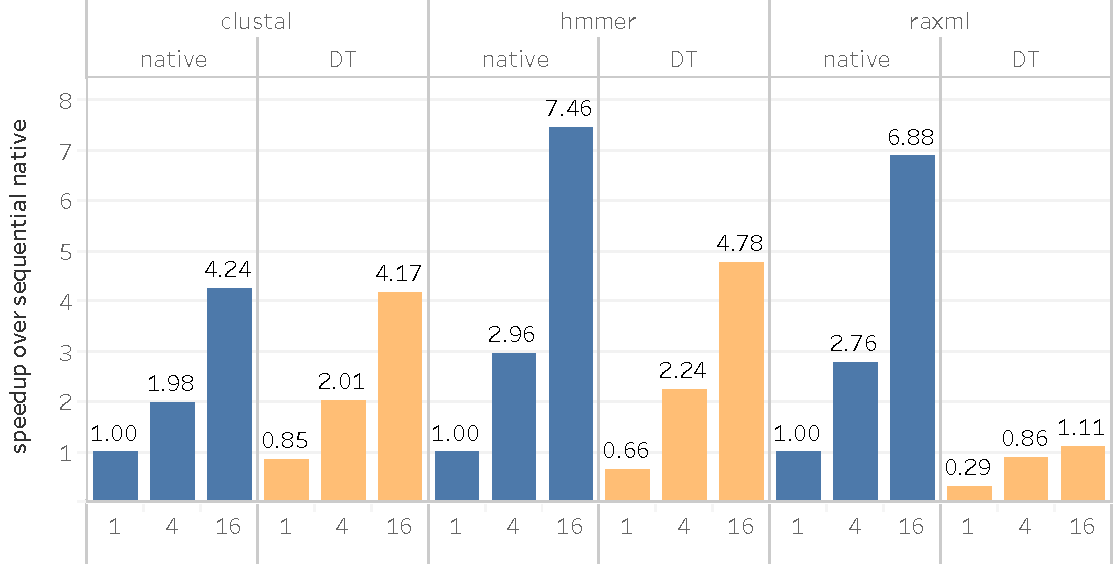
\includegraphics[width=0.95\columnwidth]{dettrace_figures/bi-scalability.pdf}
	\caption{Speedup of bioinformatics workflows with 1, 4 \& 16 parallel processes, normalized to sequential native execution (higher is better). Dark blue bars are native execution, and light orange bars are \dettrace.}
	\label{fig:bi}
\end{figure}

Our three bioinformatics workflows use process-level parallelism for performance, and exhibit a range of overheads with \dettrace, dictated by the degree to which they are compute-bound. \autoref{fig:bi} shows the speedup each workload observes with more parallel processes, normalized to sequential native execution. The highly compute-bound \code{clustal} performs the best, scaling well with additional processes and exhibiting \ClustalOverheadPct overhead with 16 processes. In contrast, \code{hmmer} and \code{raxml} execute system calls at a rate 19$\times$ higher (over 55,000/second on average), incurring more serialization. \code{raxml} in particular writes to \code{stdout} frequently, which are potentially-blocking operations that are more expensive for \dettrace, resulting in 6.2$\times$ overhead with 16 processes. \code{hmmer} has more non-blocking system calls which enable better scaling, and just 1.56$\times$ overhead with 16 processes.


\subsection{TensorFlow}
\label{sec:eval-tf}

We ran the \code{alexnet} and \code{cifar10} programs in three configurations, each of which run exclusively on the CPU: 1) natively in parallel, 2) natively but with TensorFlow configured to use a single thread and 3) with \dettrace. Since TensorFlow uses thread-level parallelism via OpenMP, \dettrace's serialized threading incurs a large slowdown over native parallel execution on 16 cores: it is \AlexnetSlowdownOverNativeParallel slower on \code{alexnet} and \CifarSlowdownOverNativeParallel on \code{cifar10}. Compared to serialized native execution, however, \dettrace fares much better with slowdowns of \AlexnetSlowdownOverNativeSerial and \CifarSlowdownOverNativeSerial, respectively, reinforcing that \dettrace exacts a small performance price for non-threaded compute-bound workloads.

% include-if-space
\begin{table}
  \begin{tabular}{ |l| r| }
    \hline
    System call events & 843,621.53 \\
    % csvstat -c DS_SYSCALL_EVENTS --mean data/sosp2019/summary_dettrace_concurrent_standard.csv
    User process memory reads & 396,474.88 \\
    % csvstat -c DS_PTRACE_PEEKS --mean data/sosp2019/summary_dettrace_concurrent_standard.csv
    \code{rdtsc} intercepted & 33,487.55 \\
    % csvstat -c DS_RDTSC_INSTRS --mean data/sosp2019/summary_dettrace_concurrent_standard.csv
    Requests for scheduling next process & 6,049.51 \\
    % csvstat -c DS_CALLS_FOR_SCHEDUING_NEXT_PROCESS --mean data/sosp2019/summary_dettrace_concurrent_standard.csv
    Replays due to blocking system call & 1,283.72 \\
    % csvstat -c DS_REPLAYS_DUE_TO_BLOCKING_SYSTEM_CALL --mean data/sosp2019/summary_dettrace_concurrent_standard.csv
    Process spawn events & 2,377.54 \\
    % csvstat -c DS_PROCESS_SPAWN_EVENTS --mean data/sosp2019/summary_dettrace_concurrent_standard.csv
    \code{read} retries & 141.28 \\
    % csvstat -c DS_READ_RETRIES --mean data/sosp2019/summary_dettrace_concurrent_standard.csv
    \code{/dev/urandom} opens & 159.92 \\
    % csvstat -c DS_DEV_URANDOM_OPENS --mean data/sosp2019/summary_dettrace_concurrent_standard.csv
    \code{write} retries & 113.98 \\
    % csvstat -c DS_WRITE_RETRIES --mean data/sosp2019/summary_dettrace_concurrent_standard.csv
    \hline
  \end{tabular}
\vspace{2mm}
  \caption{Per-package average number of events encountered by \dettrace.
  \shrink{\vspace{-3mm}}}
  \label{tab:dettraceStats}
\end{table}

% include-if-space
%\subsection{Microbenchmarks}
%% ~~~~~~~~~~~~~~~~~~~~~~~~~~~~~~~~~~~~~~~~~~~~~~~~~~~~~~~~~~~~
%
%
%Here we examine some of the worst-case overheads on particular
%instructions and system calls that are trapped by \dettrace.
%%
%First, we constructed a test harness to run the \code{rdtsc} instruction an increasing number of
%times, and, by linear regression, computed the marginal cost of adding one
%additional \code{rdtsc}, which was
%%
%8.7\nanos % Updated [2019.04.24] from Cloudlab machine c220g5-110407.wisc.cloudlab.us
%%
%running natively on one of our cluster nodes,
%versus
%% 21.1\micros
%20.1\micros % Likewise updated [2019.04.24]
%under \dettrace.
%%
%Likewise, the {\code{time}} system call slows down from
%% \textred{299\nanos to 30.2\micros.}
%238.8\nanos to 27.03\micros. % Likewise updated [2019.04.24]
%%
%These experiments perform many trials, but the R$^2$
%goodness-of-fit of the linear model was above
%%
%99\% % Likewise updated [2019.04.24]
%%
%in both the \dettrace  and native executions.
%%Because of its complex tracer/tracee context switching, we expect that \dettrace
%%would be somewhat noisier in its behavior.
%
%%\mypara{Pipes}
%% As all package builds must produce output on disk, IO is a substantial....
%%
%Most IO in package builds is through reads and writes of disk files, but to examine our
%worst-case behavior we look at pipes, which require blocking and thus create
%additional interactions with our userspace scheduler.  \autoref{fig:pipe-bench}
%shows the overhead of a ping-pong benchmark, where a message of configurable size is sent back and forth between two processes via pipes, running under \dettrace.  Once again, in
%order to measure small costs (1 byte messages) accurately, each data point
%is derived from a linear regression of roundtrip latency.
%% that estimates an exact cost for small and large times alike.
%Here we see two regimes--at smaller message sizes, we pay additional overhead
%due to higher system calls per byte transferred.


\section{Related Work} \label{sec:related}
% ================================================================================

\dettrace's unique reproducible container abstraction takes inspiration from many
previous systems. We categorize this previous work into record-and-replay
systems, and deterministic execution systems.

Many \textbf{record and replay} (RnR) systems have been proposed both from academia \cite{thomas_j._leblanc_debugging_1987,ronsse_recplay:_1999,arnold,lee_respec:_2010,castor,Dunlap:2002:REI:844128.844148,Dunlap:2008:ERM:1346256.1346273} and industry \cite{mozilla-rr,vmware-rnr,pinplay}. These systems record a trace of one nondeterministic execution to enable subsequent replay of that execution, typically for debugging purposes. These systems have broadly similar interception requirements as \dettrace, since system calls are a prime source of irreproducibility that must be recorded in the trace. \dettrace borrows some implementation techniques from Mozilla's rr \cite{mozilla-rr} as it also relies on ptrace (a quantitative comparison with \code{rr} appears in \autoref{sec:eval-rr}). Many RnR systems target multithreaded workloads, as those are very challenging to debug without RnR support, and provide high-performance parallel recording and replaying.
%
%% These systems differ in interception mechanism, ranging from binary translation
%% (PinPlay~\cite{pin-deterministic-replay}) to approaches that, like \dettrace, use
%% to {ptrace}~\cite{mozilla-rr}.
%


\textbf{Deterministic execution} schemes enforce determinism during program execution. Deterministic operating systems tackle several of the systems issues we describe in this paper, providing deterministic versions of OS abstractions like processes and threads. While Determinator \cite{amittai_aviram_efficient_2010} provides new OS abstractions for deterministic fork-join parallelism, and DDOS \cite{hunt_ddos:_2013} focuses on local network interactions, dOS \cite{tom_bergan_deterministic_2010} is closer to our work in offering a deterministic process group abstraction. The \emph{shim} abstraction in dOS bears similarity to Linux's ptrace API. Unlike \dettrace, dOS supports parallel execution of both threads and processes. However, dOS uses RnR for filesystem interactions, defining the boundaries of its determinism abstraction too narrowly to be useful for software builds which interact extensively with the filesystem. More generally, a custom OS is a heavyweight prerequisite to perform deterministic computation, and existing deterministic OSes have not evaluated portability across different microarchitectures.

% From dOS paper Section 2.1:
% ``In summary, a DPG experiences nondeterminism only when it: (1) reads data from an external source; (2) blocks to wait for external data; or (3) handles a signal sent from an external source. Our guarantee is that DPGs execute deterministically relative to a stream of such nondeterministic input, and also relative to the initial state of the DPG at the call to sys makedet. Note that this guarantee holds even across different machines.''
% jld: The cross-machine portability doesn't hold if the core count changes, and they didn't really investigate x86 features like FP insn portability, or mention cpuid at all. Being generous to them, in general dOS seems to provide roughly the same abstraction as us but at much greater complexity/fragility since it's in the kernel. Also they don't have a container component, but you could imagine them adding that. Probably they have better performance, though.

Other deterministic execution schemes focus on a single multithreaded process, determinizing interactions through shared memory. Some schemes target arbitrary binary programs \cite{devietti_dmp:_2009,coredet,derek_r._hower_calvin:_2011,devietti_rcdc:_2011,liu_dthreads:_2011,merrifield_conversion:_2013,kai_lu_efficient_2014,Merrifield:2015:HDT:2741948.2741960,Merrifield:2019:LDF:3297858.3304047}, providing generality at a modest performance overhead. Other schemes leverage language support to provide determinism for Haskell \cite{dph,eval-strategies,monad-par,lvish-popl,lvish-ppopp,concurrent-revisions-haskell} or Java \cite{bocchino_type_2009,Bocchino:2011:TRE:2032497.2032519} programs. Whether language-agnostic or specific, these approaches eliminate the influence of thread scheduling, but do not determinize IO interactions with the underlying OS and filesystem.  The scope of their guarantees is thus too small to be useful for reproducible builds. One exception is DetFlow \cite{Scott:2017:MCD:3152284.3133897} which provides deterministic parallel execution for batch jobs, though it lacks robust system call interception and requires a coordinator layer written in Haskell.

%\begin{figure}
%  %% \note{X Axis: Number of processes}
%  %% \note{Y Axis: Time to put a fixed amount of data through the whole pipeline}
%  %% \note{Variants: regular Linux and \dettrace}
%  %% \caption{Throughput of $N$ processes communicating in a chain topology through
%  %%   file system pipes.  All communications are via single-byte reads and
%  %%   writes.}
%  \centering
%%  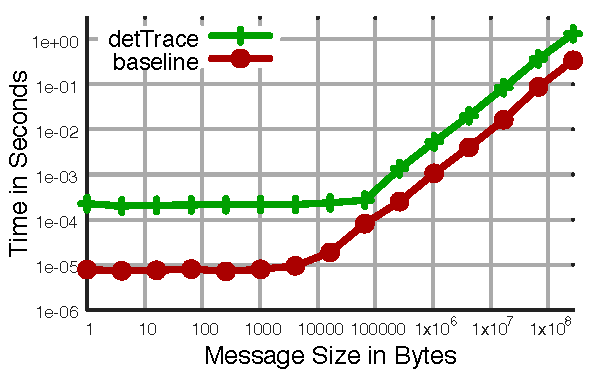
\includegraphics[width=\columnwidth]{dettrace_figures/pingpong_cutter.pdf}
%  % \vspace{-8mm}
%  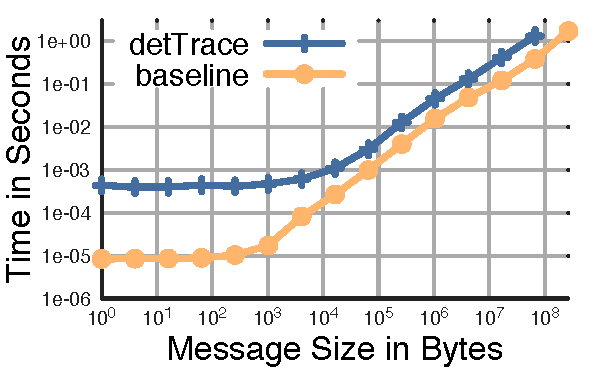
\includegraphics[width=2.5in]{dettrace_figures/pingpong_cloudlab.pdf}
%  \vspace{-3mm}
%%  \includegraphics[width=3in]{dettrace_figures/pingpong.pdf}
%  %\vspace{-5mm}
%  \caption{Amortized round-trip latency when ping-ponging messages between two
%    user processes.
%  \vspace{-2mm}}
%  \label{fig:pipe-bench}
%\end{figure}


%% FROM OOPSLA17:
%% ~~~~~~~~~~~~~~~~~~~~~~~~~~~~~~~~~~~~~~~~~~~~~~~~~~~~~~~~~~~~
%% The most closely-related work to \name are deterministic operating systems like
%% Determinator \cite{amittai_aviram_efficient_2010} and dOS
%% \cite{tom_bergan_deterministic_2010} that provide determinism for a process, or
%% a set of processes, along with the filesystem and IPC mechanisms like
%% pipes. DDOS \cite{hunt_ddos:_2013} extends the dOS system to a local network of
%% machines. While these systems provide strong deterministic guarantees, they
%% require a custom operating system which is a highly invasive change.

%% Many other deterministic systems focus solely on making shared memory
%% interactions deterministic. We divide this work into two camps: programming
%% languages that enforce deterministic parallelism, and runtime systems that do
%% so. Many of the deterministic languages are extensions to or libraries for
%% Haskell, such as Data Parallel Haskell~\cite{dph}, Evaluation
%% Strategies~\cite{eval-strategies}, monad-par~\cite{monad-par},
%% LVish~\cite{lvish-popl}, and Concurrent
%% Revisions~\cite{concurrent-revisions-haskell}.
%% %
%% Concurrent Revisions, like Determinator, takes the view that each thread or task
%% logically copies the entire heap, with changes reconciled at control-flow join
%% points.
%% %
%% Outside of Haskell, several approaches to deterministic parallelism have also been proposed, including the NESL data-parallel functional language \cite{guy_blelloch_nesl:_1992}, stream-based programming models \cite{william_thies_streamit:_2002}, type-and-effect systems for imperative languages like Java \cite{bocchino_type_2009}, and a deterministic version of the Galois system for task-based parallelism \cite{nguyen_deterministic_2014}.

%% There are also many runtime systems that focus on making programs deterministic
%% in a language-agnostic way. Some focus on programs without data races
%% \cite{olszewski_kendo:_2009}, while others focus on making even racy programs
%% deterministic via hardware support
%% \cite{devietti_dmp:_2009,derek_r._hower_calvin:_2011,devietti_rcdc:_2011}
%% or purely in software
%% \cite{liu_dthreads:_2011,merrifield_conversion:_2013,kai_lu_efficient_2014,Merrifield:2015:HDT:2741948.2741960}.
%% ~~~~~~~~~~~~~~~~~~~~~~~~~~~~~~~~~~~~~~~~~~~~~~~~~~~~~~~~~~~~

\section{Conclusions}
\label{sec:futureWork}
% ================================================================================
We have described the design and implementation of \dettrace, which provides a new \emph{reproducible container} abstraction. \dettrace automatically provides reproducibility for software builds, bioinformatics processing and ML workflows without requiring any changes to the hardware, OS, or application code. To facilitate further experimentation with \dettrace, we plan to open-source its code upon publication.

%Thus we conclude that user-space determinism enforcement is broadly useful for
%package build systems that seek bitwise-deterministic outputs.  One clear avenue
%for future work is to apply reproducible containers to the other 21 package
%managers and Linux distributions that make up the
%{\footnotesize\url{reproducible-builds.org}} project.

%Going forward, we plan to improve the generality and performance of reproducible containers, e.g., to reduce system-call interception overheads and to support parallelism. Looking further ahead, we envision reproducible containers finding many uses beyond reproducible builds. Reproducible containers can assist efforts, like the growing artifact evaluation movement, to make computer science research more reproducible. Reproducibility is a valuable property for many data analysis workflows, for validating and sharing results in the computational sciences, to enabling an audit trail for data-driven decisions taken in commerce and government. Reproducible containers can enable reproducibility in these domains with minimal perturbation to existing software.

%
%Our sequential scheduler can be generalized to support process-level parallelism in service of, \eg{} \code{make -j}. To mediate conflicts between processes, we might leverage ideas from deterministic multithreading systems.
%We could integrate \dettrace with a
%deterministic multithreading system such as Dthreads~\cite{dthreads} for
%intra-process, shared-memory parallelism (although this incurs substantial
%overheads).  Another approach for shared-memory parallelism is to integrate
%\dettrace with language-level determinism, as in DetFlow~\cite{Scott:2017:MCD:3152284.3133897}.
%In such a scenario, binaries with language-level determinism could be privileged
%to ``escape'' the sandbox and avoid overheads.
%%
%As with other sandboxes, future work can also improve the interception layer. There is substantial scope to optimize our {ptrace} usage, following the example of Mozilla \code{rr}. Another approach would be to support a Windows reproducible container using the {\em pico process} abstraction for system-call interception---the same mechanism used for the Windows Subsystem for Linux (WSL)~\cite{WSL}.
%

%% One method we've begun to explore is to sacrifice some portability and require a kernel module: \ie{} use the Dune approach~\cite{Belay:2012:DSU:2387880.2387913} to grant the user-space sandbox access to full Intel VT-x hardware-assisted virtualization support, enabling cheaper support for system call emulation and the ability to more broadly trap on instructions (like \code{rdrand}).

%


%% Finally, if reproducible containers eventually become trusted for critical
%% applications---\eg{} replicated state-machines that {\em must} stay in sync for
%% a distributed algorithm to function properly---then it will become important to
%% close any holes that adversarial programs could use to break determinism.  For
%% example, hardware-assisted virtualization methods can be used, or control-flow
%% integrity (CFI) could be enforced in user-space so that a badly behaved binary
%% cannot execute a disallowed instruction.

